\chapter{The "Stealth" Mission: "Infiltration"}

\begin{wrapfigure}{O}{\figwidth}
	\begin{center}
		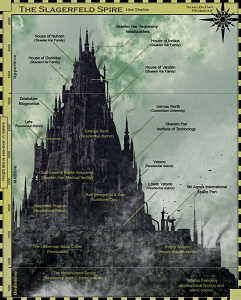
\includegraphics[width=\figwidth]{pics/18/1.png}
	\end{center}
\end{wrapfigure}
Another few hours of driving later, we discovered that the target was a "bank" in the same sense that a divisional armory is a "gun rack". 
Yes, there was something bank-like in there, and that was the part we were going to rob, but it just happened to be situated inside an entire sub-spire belonging to some sort of merchant shipping Cartel. 
This discovery did not make us very happy, and neither did the painfully long briefing we received from Sciscitat's Interrogator via combead. 


A lot of the briefing was just stuff about the Cartel, which mostly boiled down to "think Rogue Traders, except with less megalomania, more bureaucracy, and deep Administratum ties." Not being particularly interested in any of the fine details of the Cartel's sub-sector wide political connections, we strategically muted our combeads and spent most of the lecture getting some absolutely terrible "breakfast flavored" soylens wraps and fuel-station recaff. 
Eventually, possibly when she realized none of us had said anything for over half an hour, the Interrogator got to the point, which was that strange heavily armed men in shitty vans were not typically allowed on the Cartel's sub-spire. 
Unless that is, they were a PDF patrol sent to do a sweep for mutants in the sub-spire's sewers.

At first we were fine with this, we could pretend to be a PDF patrol in our sleep. 
Literally. 
The part that spoiled what was left of our appetites was where we were expected to actually go out and perform the sewer patrol. 
Sarge had suggested that the inherent laziness of PDF troopers would give us enough leeway to just sit around in our van for the whole mission without blowing our cover, but the Interrogator insisted that us fighting ravening mutants while wading through waist-deep, er, waste was a critical part of Sciscitat's plan. 
Unfortunately (for everyone involved) this turned out to be true.

\begin{wrapfigure}{O}{\figwidth}
	\begin{center}
		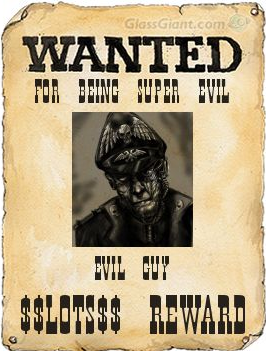
\includegraphics[width=\figwidth]{pics/18/2.png}
	\end{center}
\end{wrapfigure}
We entered the Cartel's sub-spire via its lowest vehicular entrance. 
Sarge handed the Guard in the gate-house a dataslate full of falsified credentials and orders which had been commed to Tink by the Inquisitor. 
The Guard was a bit surprised to see us, but turned up a previously unnoticed request for a PDF sewer sweep when he checked his cogitator, and accepted Sarge's grunt of "commandeered" as sufficient explanation for our non-regulation vehicle. 
He was in the process of standing down his security servitors when he suddenly got all thoughtful and asked for Sarge's name again. 


Now, our default approach to this sort of thing was to just use our own names, because honestly, why bother? 
The Imperium's a big place, and it's hard to get more faceless and interchangeable than a guardsman. 
The Inquisitor didn't see it that way though, and had issued us some "less stupid" names along with our falsified orders, and thankfully Sarge actually remembered his. 


As "Sergeant Eastwood" reintroduced himself, the Guard rooted out a piece of paper, which he held up next to the window for a second before snorting and apologising. 
When Sarge asked what for, the Guard started chuckling and handed him the paper. 
He said we could keep it, since every Astropath in the hive was handing them out and he had over a hundred.

When Sarge began emitting a high pitched wheeze the rest of us peeked over his shoulder. 
The paper was headed by the words "Wanted for crimes against the Adeptus Telepathica" and a number with a ludicrous number of zeroes. 
Below the bounty was the most cartoonishly evil caricature of a man ever seen outside of a Commissarial pamphlet. 
It was covered with scars, wearing a sinister military uniform with a stupidly oversized hat, and (with the possible exception of its grumpy expression) looked ABSOLUTELY NOTHING like "Rogue Inquisition Agent, 'Interrogator' Greg Sargent". 


We were still laughing when the Guard waved us through the gate.

\begin{wrapfigure}{O}{\figwidth}
	\begin{center}
		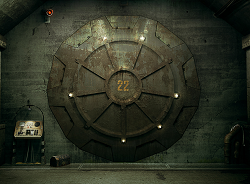
\includegraphics[width=\figwidth]{pics/18/3.png}
	\end{center}
\end{wrapfigure}
Admittedly it was impressive (and a bit worrying) that the crazy Choir Master had actually carried through with his threat and sent these wanted posters to every astropath in the sector... 
But, seriously, who goes through all that trouble and then uses an EDITORIAL CARTOON for the mugshot? 
Psykers man…

Our high spirits lasted for most of our drive through the (comparatively) clear and clean streets of the sub-spire, but faded as we reached our destination on its lowest level. 
We parked our trusty vehicle on the curb outside a maintenance station, where a pair of workers in stained coveralls met us. 
We were guided to a hatch that looked far more vault-like than your average manhole, and the grimier of the two  men promised to stay by the hatch for six hours to let us back out. 
If we weren't back by then, he said, they'd check the filtration system in about a month, and send what was left of us back to the PDF. 
While Sarge thanked the men and reviewed the few grainy vids of the mutants they supplied, the rest of did a final gear check and made sure our rebreathers were as tight as possible. 


When we got the word go, the hatch was opened, and something that looked like a cross between a man, a donkey, and a squid launched itself through the gap. 
Twitch shot it in what was probably the face, and then swore as the piddly little lasbolt failed to kill it. 
Fortunately, instead of following up the attack, the slavering mutant let out very human-sounding scream of pain and retreated. 
This didn't stop Twitch from flinging himself backwards and opening up on full auto, but the hatch-cover soaked the fire just as well as the mutant would've, so he only hit the maintenance man holding it open once. 
It turned out the guy's hand was already an augmetic so he was fairly understanding about the whole thing.

Sarge made Twitch apologise, the area under the hatch was carefully checked for any more lurking mutants, and one by one we plopped down into the muck.

\begin{wrapfigure}{O}{\figwidth}
	\begin{center}
		
\includegraphics[width=\figwidth]{pics/18/4.png}
	\end{center}
\end{wrapfigure}
Now this wasn't our first shit-slog: 
sewer patrols are a core part of what it means to be a Guardsman, and don't let any highborn stormtrooper fancypants tell you otherwise. 
It's a widely believed fact, at least among Guardsmen, that sewers magnetically attract enemies of the Imperium, and if none are present to be attracted, will just spontaneously generate them out of thick air. 
Why this happens is a mystery which eludes even the most unqualified barracks scholars. 
Maybe it's something to do with the universal vacuum hatred thingy, or maybe there's actually something to that line in the Primer about how "filth breeds filth". 
In any case, the important part is that leaving a sewer unpatrolled will inevitably wind up biting you in the collective ass, sometimes literally. 


Back in the Guard, long standing tradition dictated that the least senior regiment on the battlefield (which always seemed to be ours for some reason) got the fun job of going down there every few days to clear out the latest infestation of greenskins. 
Or heretical cultists. 
Or genestealers. 
Or gangers, carnivorous plants, secessionists, mutated housepets, deserters, rogue servitors, previously unidentified intelligent xenos races, dead gods, or cannibalistic humanoid underground dwellers… It was sort of like a lottery: 
you never knew what you were going to get when you went down, except you sort of did, because nine times out of ten it was Orks. 


Fortunately, the Cartel's sewers were one of those rare Ork-free ones, and it turned out that the horrific mutants which did inhabit it were a lot less suicidally aggressive than your average greenskin. 
Well, at least the humanoid ones were: 
we did encounter some unusually sized rodents which were, in Twitch's words, "suspiciously similar" to squigs. 


\begin{wrapfigure}{O}{\figwidth}
	\begin{center}
		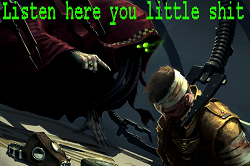
\includegraphics[width=\figwidth]{pics/18/5.png}
	\end{center}
\end{wrapfigure}
Anyway, the majority of the sewer's occupants wanted to get shot about as much as we wanted to get shivved with a piece of sharpened fecal matter, and we quickly came to a mutual understanding with them. 
This wasn't anything official mind you, the presence of Cartel security monitors meant we couldn't just announce that we were just passing through on a secret Inquisitorial mission, but we managed to convey the gist of it by making as much noise as possible, waving our lights around, and loudly announcing the complete lack of mutants we were seeing. 


So, by the standard of armed patrols through ass-deep (or neck-deep in Nubby's unfortunate case) sewage, it was a fairly pleasant experience. 
Or it would have been if it weren't for the Inquisitor's fetish for overly complicated plans. 
He'd put together this amazingly complex series of carefully timed infiltrations, misdirections, psychic tricks, and cogitator infiltrations, which was supposed to result in them nicking the doohickey without the Cartel even finding out they'd been robbed. 
We were fine with all that, it wasn't like we wanted to get into a shooting war with someone who could afford to employ entire goon-battalions, and our part was actually pretty simple. 
All we had to do was to sneak into one of the sub-spire's auxiliary power stations via the sewers and do something technical to some sort of feed line thingy. 
Honestly, we were a little hazy on the fine details, but Tink claimed it was all "super simple", which was good enough for the rest of us.

The problem was that, for some reason, the Inquisitor didn't trust us to get our part done unsupervised. 
Which is why, instead of just giving us a map and the codes to the security doors, we were being guided through the sewers via combead. 


By the tech-priest. 


The one who hated us.

\begin{wrapfigure}{O}{\figwidth}
	\begin{center}
		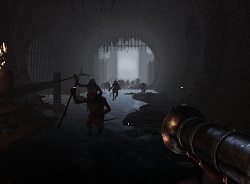
\includegraphics[width=\figwidth]{pics/18/6.png}
	\end{center}
\end{wrapfigure}
We bore the constant stream of insults, slanders, and reminders that our sins against the machine god had damned us to an eternity of torment in the unholy scrapyard of lost souls or whatever without complaint. 
What was harder to ignore though, was the way our directions seemed to guide us unerringly right through the middle into every single dangerous, disgusting, inconvenient thing in the entire sewer system. 
Call it the kneejerk paranoia of a bunch of jumped-up jarheads, but by the third time he sent us directly into a nest of mutated rat things, we were fairly certain he was trying to get us all killed. 


Of course, consummate professionals that we were, we put up with the tech-priest's shenanigans. 
After all, it wouldn't do to disrupt the Inquisitor's plan and put both the objectives and our beloved comrades at risk over something as minor as a bit of degradation and danger. 
Also, the metal bastard had control over the only external channel our combeads could reach from down in the sewers, so our choices were a bit limited. 
In any case, as guardsmen we were quite familiar with suicidal orders and knew how to deal with them, so it was more of an annoying inconvenience than anything.

Through a combination of lying, paranoia, undisclosed scouting, and creative interpretation, we made it to the section of sewers which paralleled the power substation's maintenance tunnels without any serious cock-ups. 
Admittedly Tink and Twitch were going to need to need a whole lot of immune-boosters for the scratches they'd received from the second rat nest, and Nubby had been submerged to the point where even he agreed that a bath was needed. 
Doc was just incredibly thankful for the purge valves on his rebreather after some sort of tentacle thing ripped it off long enough for the smell and subsequent nausea to set in, and Sarge was a simmering pot of barely-contained rage over the whole situation, but we reached the target on schedule and in piece. 
More or less.

\begin{wrapfigure}{O}{\figwidth}
	\begin{center}
		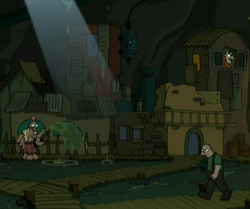
\includegraphics[width=\figwidth]{pics/18/7.png}
	\end{center}
\end{wrapfigure}
Getting into the power station's maintenance tunnels turned out to be a bit of a problem. 
This was partially because the people who ran the place had put quite a lot of effort into separating the vital heart of their sub-spire from the mutant-infested sewers adjacent to it. 
Mostly though, it was because the tech-priest kept insisting the only possible entrance was located in a chamber which just happened to contain an entire mutant village, complete with hovels, barricades, and what looked to be a sizable militia. 
When Sarge pointed this out to the tech-priest, he just made a suspiciously snicker-like sound and asked how that was HIS problem. 


After a brief debate, we decided that there was no way in hell that we were going to try fighting our way past seventy-ish spear-carrying mutants, and an alternative approach was needed. 
We spent a bit of time searching the immediate area for likely-looking passages and checking the map Tink had been compiling (so we could navigate our own route back, thank you very much), but weren't making much progress until Doc suggested just asking the Mutants if they'd let us through. 
The rest of us, especially Twitch, thought this was a bit overly optimistic, but there wasn't any real harm in asking, so Sarge approached to what he felt was just beyond spear-chucking range and committed diplomacy.

To our considerable surprise given Sarge's diplomatic track record and all, things actually went pretty well with the mutants. 
As it turned out, not only did a few of the mutants know how to speak a sort of horrible gargly version of Gothic, they were also fairly well disposed towards us on account of how much effort we'd gone through not to fight them. 
"Well disposed" isn't the same as "stupid" though, so they weren't keen on the idea of letting a bunch of armed goons pass through their village, but once Sarge explained our destination they were more than happy to point us towards an alternate entrance to the maintenance tunnels.

\begin{wrapfigure}{O}{\figwidth}
	\begin{center}
		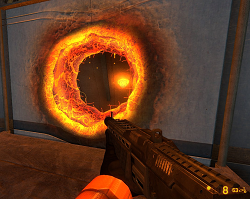
\includegraphics[width=\figwidth]{pics/18/8.png}
	\end{center}
\end{wrapfigure}
Despite Twitch's insistence that the mutants were sending us into a trap, we followed their directions to a small security door without incident. 
Unfortunately, there was a slight holdup at this point, because when we asked the tech-priest for the access code he immediately figured out we were at a different door, and kept trying to send us back through the mutants to the "correct" one. 
When Sarge refused to budge without an explanation, the contrary cogboy told him that the door we'd found connected to an entirely different facility. 
Tink, who'd discovered a dataport next to the door and had (without asking for permission or sparing the slightest bit of thought for all the bad things that might happen) immediately plugged his dataslate into it, announced that he'd found a map of the power station and that we were only three rooms and a short hallway from the target. 
The tech-priest immediately backpedaled, declaring that the REAL problem was that he didn't have an access code for this door; 
Sarge told him we'd just cut our way through it then.

After a few more go rounds with the tech-priest, in which he tried to convince us that the door was monitored, booby-trapped, a secret portal to the eye of terror, etc. 
and we checked his assertions and found them to be a load of bullshit, Tink set his plasma gun to "cut". 
The home-converted astartes pistol, which had not originally had any such setting, immediately vented a stream of superheated gas in the general direction of Tink's face and was dropped into the ankle-deep muck at his feet. 
After three more failures, and a lot of complaints about how it'd been working earlier and how much better his Tau-ified weapon had been, Tink admitted defeat and just shot the thick door until a sizeable hole had been slagged through it. 
After cooling the hole with the readily-available resources, we squeezed through into the power station.

\begin{wrapfigure}{O}{\figwidth}
	\begin{center}
		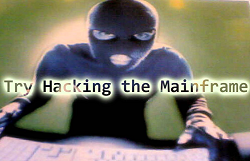
\includegraphics[width=\figwidth]{pics/18/9.png}
	\end{center}
\end{wrapfigure}
The room on the far side of the door turned out to be one of those weird mechanicus combination shrine and control room dealies. 
As we tracked sewage over cogboy-themed religious icons and the occasional piece of delicate machinery, it occurred to us that the tech-priest might've had an actual reason for not wanting us to come this way. 
Not that any of us particularly cared, but it did shine a bit light on why he was screaming at Sarge loud enough for the rest of us to hear him despite our muted combeads.

Sarge, being aware that there was probably a limit to how many doors we could breach before triggering an alarm, announced a short halt to see if the furious cogboy was going to calm down enough to start giving directions again. 
Twitch, Nubby, and Doc respectively used this time to barricade the door behind us, nick the candlesticks, and wipe off as much filth as possible at the expense of a tapestry depicting the discovery of a new type of toaster by Tech-Saint Gearface. 
Despite his personal tendency towards tech-heresy, Tink didn't join the rest of us in desecrating a holy mechanicus shrine. 
Instead, the techie wandered over to the main control altar, and after a few seconds of translating cogboy glyphs, excitedly informed the rest of us that he could use it to disable a thing, overload another thing, and start some sort of cascade. 
When the rest of us just stared blankly at him, he explained that this would automatically trigger the thing which the Inquisitor had sent us down here to do. 


Sarge was a bit dubious, and claimed to remember our orders involving going to the main transformer room and doing something a bit less catastrophic sounding, but Tink maintained it would have the same end result. 
Probably. 
That is, assuming "logical" failsafe design. 
And good maintenance practices. 
And none of the capacitors being too full. 
And no stupid machine spirit shenanigans.

\begin{wrapfigure}{O}{\figwidth}
	\begin{center}
		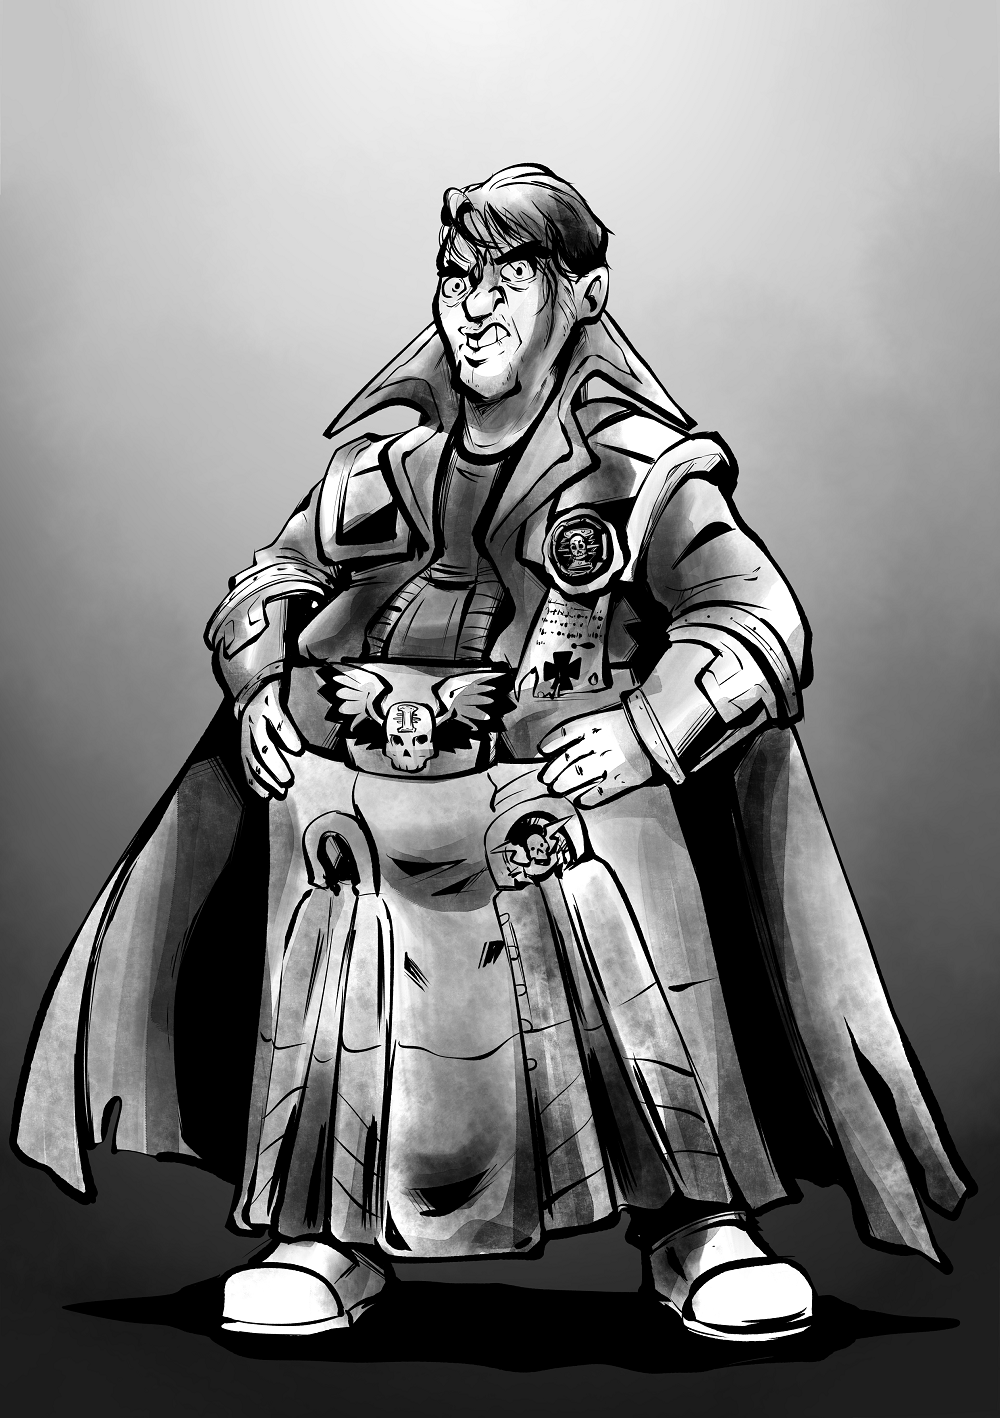
\includegraphics[width=\figwidth]{pics/18/10 large.png}
	\end{center}
\end{wrapfigure}
Sarge decided to make "potentially blow up the power station we've just infiltrated" Plan B, and informed the tech-priest of it in an attempt to get him to start cooperating with Plan A. 
The threat didn't have as much effect as we'd hoped: 
it turned out that while we'd been ignoring him the cogboy had managed to find a vid feed of the shrine and was practically frothing at the lips over our actions. 
Or, y'know, would've been if he'd had lips. 
Anyway, he wasn't in the mood to be helpful, but fortunately the Inquisitor chose that moment to join the comm channel and check what our ETA was; 
Sarge gleefully threw the enraged tech-priest under the proverbial armored personnel carrier.

Showing his usual lack of tact, Sciscitat decided to chew out the tech-priest on the open channel. 
It'd be a lie to say we didn't enjoy listening, and maybe the tech-priest had enough awe for the Inquisitor's supposed genius that he wasn't going to hold a grudge towards him, but we were fairly certain the experience pushed his irrational hatred of us to whole new levels. 
For the time being though, the lecture did the trick, and the tech-priest grudgingly began opening doors, disabling vid feeds, warning us of servo-skull patrols, and providing non-bullshit directions. 
While the route he sent us down was a little less direct than the one Tink's map suggested, there seemed to be actual reasons for the detours this time, so we kept our mouths shut and advanced into the heart of the power station in as professional a manner as possible for five men covered head-to-toe in shit.

\begin{wrapfigure}{O}{\figwidth}
	\begin{center}
		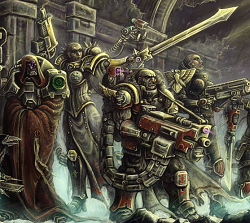
\includegraphics[width=\figwidth]{pics/18/11.png}
	\end{center}
\end{wrapfigure}
We eventually entered the target, "Distributor Room C", via a small conduit-filled tunnel and found ourselves on a raised catwalk above a room full of large, occasionally sparking machines which we assumed were the distributors. 
Thanks to our aerial perspective we didn't have any trouble finding the machine which controlled the power flow to the upper levels of the Cartel's sub-spire, and Tink was easily able to identify the control altar on it that he needed to sabotage. 
The problem was that said control altar was currently in use. 
By another Inquisition team.

It was a bit an awkward situation. 
We considered going down there and asking them if their super secret mission was going to take very long, and if they wouldn't mind if we snuck in ahead of them, but we got the feeling that wouldn't go over well, so in the end we decided to kick the problem upstairs. 
To nobody's surprise, it took a few tries to get the tech-priest to patch us through. 
He was a bit leery of our identification of a bunch of random people in our way as a highly trained Inquisition team that just happened to be infiltrating the exact same facility at the exact same time as us, and suggested that they might just be a simple maintenance team and we might just be a bunch of paranoid idiots. 
Sarge rather sarcastically pointed out that the "maintenance team" consisted of a combat-auged tech-priest with a pair of gun-servitors, a mohawk-sporting underhive Ganger carrying her bodyweight in firearms, and a Sister of Battle in full body armor. 
Honestly, and some people accuse US of being unsubtle…

The tech-priest was very obviously in the middle of trying to figure out a scenario where we could still be wrong, when the distributor-thing the other team was messing with let off a massive bolt of electricity, the lights went out, and Sciscitat cut into the channel himself with a screech about how we'd reset the thing too early and had nearly killed three of our teammates.

\begin{wrapfigure}{O}{\figwidth}
	\begin{center}
		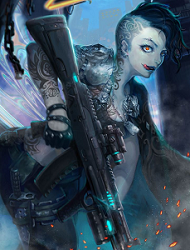
\includegraphics[width=\figwidth]{pics/18/12.png}
	\end{center}
\end{wrapfigure}
To Sciscitat's credit, he stopped his ranting about how we were the most relentlessly incompetent jackasses to ever enter Inquisitorial service mid-insult when Sarge mentioned the second team. 
The man shifted mental gears with impressive speed, and began barraging us with questions about what the three people below us were doing, saying, wearing, and whether we recognized them from the dossiers of known Conspiracy agents we'd be shown. 
Sarge glibly reminded him that we hadn't been shown anything, before ordering Tink, who was the only one of us who could see in the dark without the aid of a flashlight, to peek over the edge of the catwalk. 


While Tink and Sarge relayed a whole lot of unhelpful information to an increasingly annoyed Sciscitat, the rest of us fanned out into good firing positions. 
It wasn't that we *wanted* things to devolve into a bloodbath, it was more about being well prepared, not to mention realistic. 
Anyway, Tink really did try to give the Inquisitor the intel he wanted, it was just that nothing he reported seemed to be useful to the man. 
The Ganger's weapon collection didn't interested him, and neither did the fact that the Sister was fucking huge by anything but Space Marine standards (seriously, she probably had a head on Sarge out of her armor). 
Tink's attempts to convey the techy features of the cogboy didn't go any better, and before long Sciscitat disconnected in a completely unjustified huff, leaving us all standing there with absolutely no idea what to do.

Well, for a few seconds at least. 
The question of whether the people below us were Conspiracy agents or just another Inquisition team with a terrible sense of timing suddenly became moot as the underhive Ganger below us, who'd been mocking the tech-priest in a very Aimy-like way, asked the big Sister what smelled like the concentrated essence of a thousand asses. 
Tink and Sarge pulled back as the sniffing Ganger directed her tac-light upwards, but not quite fast enough.

\begin{wrapfigure}{O}{\figwidth}
	\begin{center}
		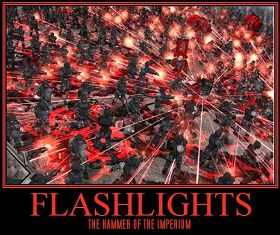
\includegraphics[width=\figwidth]{pics/18/13.png}
	\end{center}
\end{wrapfigure}
Fortunately for Sarge and Tink, the catwalk was a sturdy sheet of metal instead of some flimsy grated surface, and easily withstood the hail of stub rounds sent their way by the Ganger. 
The Sister and her bolter were another matter though. 
The pair of troopers sprinted across the catwalk just ahead of a line of shrapnel-spraying craters, only barely managing to make it behind a big support pillar before they were hit. 
The rest of us unanimously decided that there wasn't any more time for dicking around about whether the people below us were dirty traitors or just misguided homicidal assholes, and opened fire on the two gun-servitors before they could bring their heavy weapons to bear on Sarge and Tink's position.

Despite the relative piddly-ness of standard lasguns, a triple helping of pre-aimed, braced, and full-auto bolts on each was enough to put both servitors down. 
The one armed with a heavy bolter just keeled over as its metal-filled skull popped, but the plasma-gun armed one went off with a very satisfying bang, tossing the nearby tech-priest backwards and thoroughly wrecking the control altar. 
This caught the attention of the Ganger and Sister, who both switched to laying down suppressive fire while moving to pick up their damaged cogboy. 
This was a terrible choice on their part (as any of us could have told them) since even with the Ganger firing a weapon with each hand and them both fanning their fire back and forth in an attempt to cover all of us, it still left their backs open to Sarge and Tink.

\begin{wrapfigure}{O}{\figwidth}
	\begin{center}
		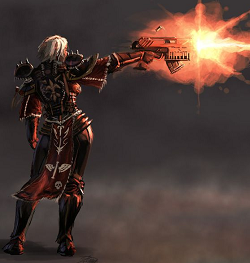
\includegraphics[width=\figwidth]{pics/18/14.png}
	\end{center}
\end{wrapfigure}
Despite his efforts to tweak the weapon, Tink's "gifted" plasma pistol didn't have the same range or reliability of his old gun, which is why the Sister survived his opening barrage with only a damaged power-pack and helmet. 
Sarge might've done better with the Ganger, but the shot he was lining up on her head was interrupted by an ear-splitting shriek from his combead. 
Sciscitat, who was none too happy that we'd been ignoring him in favor of staying alive, demanded an update and promised us horrible deaths if we failed to take at least one of our opponents alive. 
Sarge briefly considered how likely the Sister or Tech-Priest were to cooperate with something like that, regretfully shifted his aim downwards, and shot the Ganger in her ammo-filled cargopants.

As the Ganger dropped screaming all five of us focused our fire on the Sororitas. 
To our considerable surprise given our past experience with crazy battle-nuns, instead of battle-hyming her way to a heroically stupid death, the big Sister just walked out on us. 
Seriously, she didn't even run, her only concession to our presence was to fire a few scarily well aimed shots in Tink's general direction before grabbing her Tech-Priest by the leg. 
She tossed the groggy cogboy through the nearest exit, tucked the wounded Ganger under one arm, sprayed a few more shots Tink's way, and then almost nonchalantly WALKED OUT. 
Just letting her armor soak our lasfire until the hallway blocked our line of sight. 
It was a bit embarrassing really.

\begin{wrapfigure}{O}{\figwidth}
	\begin{center}
		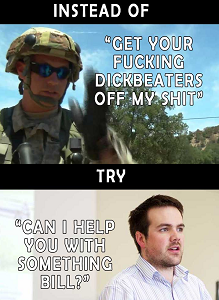
\includegraphics[width=\figwidth]{pics/18/15.png}
	\end{center}
\end{wrapfigure}
Our embarrased shock at the situation was interrupted by the sound of a heavy security door beginning to close behind the hostile team. 
Thinking fast, Nubby and Twitch both shot the door's control panel. 
Thinking a bit less fast, but a whole lot harder, Tink sprinted out from the secure cover he'd been cowering behind and managed to put a pair of shot's into the servos controlling the door, which proved to be a lot more effective. 
Before the techie could smugly point that out to anyone though, one end the bolter-cratered catwalk he'd run out on gave way with a grinding screech. 
Lacking any better way to get to ground level, the rest of us scrambled down the makeshift ramp after him.

Sarge made it to the half-closed door first, and sprang back from it with a curse as a pair of autogun rounds hit him in the helmet and chestplate. 
Neither round penetrated fortunately, at least not much, but it was enough to convince him to wait for the rest of us. 
A few seconds later Twitch tossed through one of our limited supply of flash grenades and we scrambled into the hallway weapons ready just in time to see a side-door slam shut. 
Sarge swore as the door's control panel emitted a burst of binary and flashed a bright red cog icon, told Tink and Twitch to either unlock it or breach it, and took a second to address the increasingly angry noises coming from his combead. 
Doc and Nubby snickered has he told the Inquisitor we were "handling it", asked him to stop bothering us, and suggested that if he wanted us to stand even the slightest chance of catching the other team, much less capturing one of them alive, to have our useless ass tech-priest undo whatever theirs had done to the door.

The Inquisitor didn't enjoy being told to cram a sock in it, but after a few seconds of yelling the door sprang open. 
This surprised the hell out of Twitch and Tink, who dove into cover on the far side a split second ahead of a hail of bolts, autogun rounds, and bright-blue las-fire.

\begin{wrapfigure}{O}{\figwidth}
	\begin{center}
		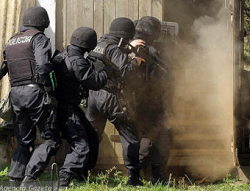
\includegraphics[width=\figwidth]{pics/18/16.png}
	\end{center}
\end{wrapfigure}
If you haven't ever had to advance cover-to-cover under fire, rest assured that it isn't a fun experience. 
The one upside was that the other team was probably having just as miserable a time trying to escape us as we took shots at their backs. 
Fortunately for both us and them, the hallway was littered with inexplicably convenient cover in the form of pipes, conduits, and doorways.

Chasing the probably-traitors proved remarkably difficult. 
The Ganger, who was now limping along instead of being carried, poured out a steady stream of heavy stubber, then autogun, then hand-cannon rounds in a poorly aimed barrage. 
The tall Sororitas calmly walked backwards down the hallway at a leisurely pace, dedicating the entirety of her fire to whichever cover Tink had chosen. 
The techie still managed to get a few shots off with his modified plasma pistol, but none of them scored more than a glancing hit, and after a particularly near miss sprayed shrapnel across his neck and shoulders, he decided that not dying took priority over pot-shots. 
The rest of us poured quite a bit of fire into the Sister's power armor while she walked between cover, but it proved frustratingly ineffective. 
In retrospect, we probably should've focused our fire on the injured tech-priest rolling up the corridor ahead of her.

Our advance up the corridor was interrupted twice, first by a pair of tech-priests who opened a door where Twitch and Doc were taking cover. 
Twitch shot one of the approaching cog-boys in the gut on reflex, and there was an awkward moment as Doc and the second tech-priest apologized at each other before the door was closed again. 
The second interruption was far more problematic. 


\begin{wrapfigure}{O}{\figwidth}
	\begin{center}
		
\includegraphics[width=\figwidth]{pics/18/17.png}
	\end{center}
\end{wrapfigure}
We'd steadily gained on the enemy team thanks to our innate guardsmanly ability, plus the fact that two of them were wounded and the third seemed dead set on walking everywhere. 
Sarge was actually entertaining the thought that we were going to be able to pull of our ordered capture, when one of the two doors at the end of the corridor opened to disgorge a pair of servitors and a trio of servo-skulls. 
The damned tech-priest screeched something and the whole group began lurching and hovering towards us prompting Sarge to declare that Shit Was Fucked: 
it was time to pop nades and end this, regardless of what the damned Inquisitor wanted.

An expertly-aimed barrage consisting of two frags and a krak sailed forwards to wipe out the enemy team before they could escape; 
unfortunately, the tech-priest saw them coming. 
Sarge, Nubby, and Twitch's expressions abruptly changed from grim satisfaction to alarm as their own grenades, gripped firmly in the jaws of the three servo-skulls, zoomed back towards them. 
The three troopers began frantically backpedalling and firing at the suicide skulls, and then switched to a full panicked sprint as their shots missed and the skulls gained even more speed. 
It was only a few well-aimed shots from Tink and Doc, who were far enough back to put their full attention into firing, that prevented outright disaster. 
The two skulls carrying frags were knocked out the air and went off behind some obstructing pipes, while the one with Twitch's shorter-fused krak detonated short of its target. 
Twitch, Nubby, and Sarge were pelted with a fragments of red-hot metal and bone, but their armor protected them from the majority of it and they climbed back to their feet with only superficial injuries.

\begin{wrapfigure}{O}{\figwidth}
	\begin{center}
		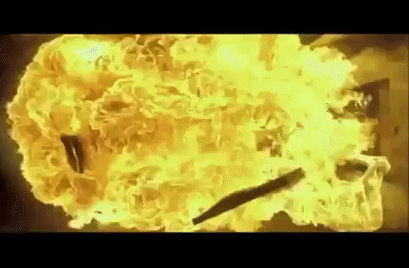
\includegraphics[width=\figwidth]{pics/18/18.png}
	\end{center}
\end{wrapfigure}
Unfortunately, that little grenade misfire ate up several crucial seconds of our attention. 
When the smoke cleared we found the two maintenance servitors blocking our line of sight to the fleeing team. 
We tried to catch back up while Tink burned down the obstructing servitors, but before we could get a clear shot or reach grenade range again, the three hostile agents staggered through the door the servitors had come from. 
Sarge and Twitch managed to snap off a few shots as it closed, but failed to hit anyone but the stoic Sister, who didn't even bother turning to return fire (the Ganger however hurled a few amazingly creative insults and flipped us all off). 


As the door slid shut with a little *ding* it occurred to us that the room behind it had looked rather elevator-like; 
Sarge swore and keyed his comm to ask whether our tech-priest could stop the thing while the rest of us climbed over the remains of the servitors and raced towards the second elevator next to it. 
We were about five meters from it when there was an odd metallic sound from somewhere above us and both elevator doors rattled slightly. 
We all slowed down and readied our weapons, just based on the theory of general paranoia, but didn't really grasp what had just happened until Tink noticed the rapidly descending floor number. 
Twenty-five seconds of all-out sprinting got us to the far end of the hallway, through the door, and halfway back to the distributor room before the second freight elevator crashed into the bottom of its shaft at terminal velocity. 


In the ringing silence that followed, the Inquisitor finally answered his comm and asked us if we'd caught them yet. 
He wasn't very happy with our answer.

\begin{wrapfigure}{O}{\figwidth}
	\begin{center}
		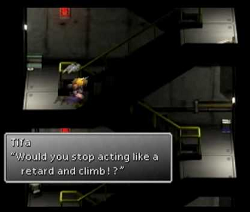
\includegraphics[width=\figwidth]{pics/18/19.png}
	\end{center}
\end{wrapfigure}
We got the impression that Inquisitor Sciscitat dearly wanted to strangle us with his bare hands, or failing that, to dedicate a proper few hours to chewing us out. 
Judging from all the chatter we could overhear on his line though, he was a tad too busy for either. 
After a few enraged sputters, he bitterly declared that he didn't have the time or crayons to explain the degree to which we'd failed him, told the tech-priest to get us up to the bank before the shooting started, and closed the channel. 
As the cogboy rather smugly directed us down a side corridor, we overheard the Inquisitor telling the rest of the team that "the idiots have done it again" and to enact Contingency Plan Theta-Seven or something. 
We made a few choice remarks of our own, but didn't bother transmitting them.

We sprinted through the maintenance tunnels, hurrying to join our comrades up in the bank and regain our lost honor on the field of battle. 
Well, at least we started to, but then we got to the stairs and realized that we were currently on "Level -57" and our destination was on "Level 184". 
How either the Inquisitor or the tech-priest expected us to not only climb over two hundred flights in less than thirty minutes (wearing full armor and rebreathers no less) AND THEN go directly into combat… We took one look at those stairs and unanimously decided to go back to the van and just find a way into the bank from the outside.

The tech-priest wasn't happy with our unilateral decision, or what we told him to do with his directions, and loudly declared that he had more important things to do than guide us back through the sewers. 
Sarge told him that suited us just fine and suggested he go do those better things. 
The Inquisitor was called in to yell at us, but things were evidently getting hectic upstairs, because he just to told the tech-priest not to waste time "wrestling with pigs" (whatever that meant) and both of them finally stopped bothering us.

\begin{wrapfigure}{O}{\figwidth}
	\begin{center}
		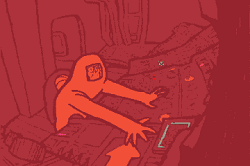
\includegraphics[width=\figwidth]{pics/18/20.png}
	\end{center}
\end{wrapfigure}
As we retraced our path the sub-spire's maintenance tunnels, completely ignoring stealth this time and just pre-emptively shooting any servo-skull patrols we saw, Twitch put forward the question of setting up "distractions". 
After all, we'd be going right through that fancy control-shrine place, right? 
Tink's eyes lit up with downright evil light, and he, Nubby, and Twitch all started giggling. 
Sarge and Doc shared a look, remembering past lectures on collateral damage and keeping a low profile, but didn't raise any objections.

We re-entered the shrine to find it occupied by a tech-priest, who screeched something about "blasphemers" and drew a side-arm, which was the last mistake he ever made. 
Tink and Twitch shifted the idiot's remains and went to work on the controls, turning pretty much every one of them to either the max or minimum. 
By the time the rest of us had finished moving our anti-mutant barricade to block any meddling cogboys from entering about seven different alarms were blaring and a small statue of some saint or other was screaming at us in binary. 
Tink slagged two of the control altars with a last gleeful cackle, we snugged up our rebreathers, and made our way back out into the sewers.

It turned out that the barricade had actually had a purpose, because we found a bunch of those non-confrontational mutants hanging around outside. 
Twitch nearly shot one, but Sarge and Doc managed to keep things from devolving into a bloodbath and we just sort of awkwardly sidled past them. 
Tink called back advising them to, in his own words:

>"Get, I dunno, like half a klik away before the first capacitors go. 
Not EXACTLY sure how long you got, but unless you're fire or electricity-proof, and I'm not ruling that out 'cause you guys are fuckin weird lookin, but I really wouldn't recommend sticking around if you don't got them both covered. 
Oh, and there's gonna be a lot of REALLY angry cogboys coming down here afterwards, so, uh, have fun with that."

\begin{wrapfigure}{O}{\figwidth}
	\begin{center}
		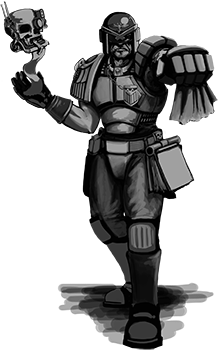
\includegraphics[width=\figwidth]{pics/18/21.png}
	\end{center}
\end{wrapfigure}
Using the map we'd compiled ourselves instead of the tech-priest's oh-so-helpful directions, backtracking through the sewers went a hell of a lot smoother. 
We reached our entrance with only two shots fired, and while we did pick up a fresh coating of muck, it only reached our knees this time, thank the Emperor. 
We knocked on the hatch and were let in almost immediately by the two maintenance guys, who seemed surprised to see all of us still alive and in possession of all of our limbs. 
They had a lot of questions about how things had gone and if we'd seen any mutants messing with power conduits, but Sarge told them we'd file an official report when we got back to PDF HQ and led our not-quite-run back out to the van.

When we were about halfway out of the building our combeads finally reconnected to our team's non-boosted channels and we suddenly got a far better idea of how much shit was going down. 
The tech-priest and Snitch were calling out all sorts of warning about Cartel security movements and the position of the rest of the hostile Inquisition team we'd encountered. 
Face and the Assassin were halfway into some vault, but were worried about some flier that had just landed. 
The Cleric and Interrogator were dodging patrols while trying to get to somewhere ahead of the other team. 
Sciscitat was in the middle of this all, calling out a constant stream of orders intermixed with vague curses about "greedy idiots", "traitors", and "incompetents who couldn't follow an order if their lives depended on it". 
We assumed the last one was directed at us. 


Sarge was debating whether to check in now, or put the inevitable screaming lecture off until we'd driven up to the bank, when he caught sight of the van and stopped dead. 
The rest of us peeked around him and started swearing as well as we saw the thick papering of traffic tickets covering our vehicle, and the singed, bleeding, vindictively glaring Traffic Officer standing in front of it.

\begin{wrapfigure}{O}{\figwidth}
	\begin{center}
		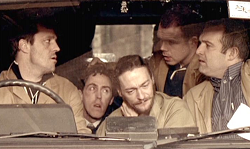
\includegraphics[width=\figwidth]{pics/18/22.png}
	\end{center}
\end{wrapfigure}
Our paralysis only lasted for a moment. 
Without a word or signal, every one of us reached the same conclusion: 
there was not time for this shit. 
Sarge strode forward in a calm, unhurried manner, staring directly into the Officer's visor the entire time. 
When they were only a pace apart, Sarge wordlessly held out his right hand for the ticket the man had been writing; 
his left hit the Officer in the jaw with the concentrated force of an entire mission's worth of pent-up frustration. 
Also, brass knuckles. 
Spikey ones.

Despite the bone-crushing force of Sarge's sucker punch, between the ex-Arbite's full helmet and his own considerable burliness the man actually managed to stay on his feet and started to reach for his weapons. 
We'd counted on him being a tough bastard though, and Sarge's hit was followed up by an augmetic leg to the groin and a blow from Tink's shock-wrench. 
As the Arbite started to crumple Doc and Twitch grabbed him by the arms, heaved him into the rear of our van, and piled in after him.

There was a lot of thumping and cursing from the back of the van as Tink weaved our vehicle steadily upwards through the sub-spire's light traffic. 
By the time we were approaching the upper levels our "guest" had been relieved of his gear and weapons, jabbed with three syringes of sedative, and covered from mouth to feet with a dozen layers of duct-tape. 
This was just a temporary solution of course; 
Nubby suggested a more permanent one involving the nearest edge of the sub-spire, which Doc objected to for silly moral reasons. 
Twitch insisted that the Officer had some sort of power that would keep him coming back unless we actually watched him die ourselves, and then exploded the body. 
Sarge quashed further discussion on the subject: 
as far as he was concerned deciding what to do with the annoying Traffic Officer could be the Inquisitor's problem. 
For now he could just take a nice relaxing nap in the back of the van until we'd finished our mission.

\begin{wrapfigure}{O}{\figwidth}
	\begin{center}
		
\includegraphics[width=\figwidth]{pics/18/23.png}
	\end{center}
\end{wrapfigure}
To nobody's surprise, when we informed the boss that we'd reached the topmost level of the sub-spire and needed directions to our entry-point, we got yelled at for how long it'd taken us. 
This completely disregarded the fact that if we'd gone up the stairs we'd have still only have been about halfway up, but by that point we'd given up on expecting reasonable reactions. 
When Sciscitat finished venting, he directed us to the side street where the scan-van was parked. 
We were told to park our vehicle, meet up with Snitch (who would be both our guide and escortee), and gear ourselves up for a fight.

We got a lot of worried looks from the Cartel merchants and scribes walking the street as we piled out of our van. 
This wasn't that surprising given that we were in full armor, carrying as much ammo, explosives, and situational toys as we could, and still covered in a not-quite-dry layer of fecal matter. 
What WAS surprising was that nobody ran screaming or called the Cartel's security force the second they saw us, not that we were complaining, but either they had way too much faith in their outer-perimeter or one of our teammates had done something impressive to explain-away our presence. 
We tried to ask Snitch which it was as he hopped out of the scan-van and led us to a nearby service door, but greasy little weasel was more interested in complaining about our smell and asking why we kept thinking about some Arbite. 
We decided that conversation could wait for later, and resolutely thought about other things until the service door slid open and let us into yet another set of maintenance tunnels.

\begin{wrapfigure}{O}{\figwidth}
	\begin{center}
		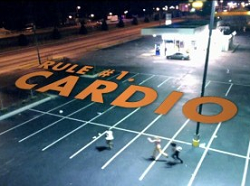
\includegraphics[width=\figwidth]{pics/18/24.png}
	\end{center}
\end{wrapfigure}
The building we'd entered wasn't the Bank, but thanks to the interconnected nature of hive construction and our teammates' apparently total control over all automatic doors in the area, that really wasn't a problem. 
Snitch led us down several suspiciously empty tunnels and into a familiar massive stairwell, but the whiny psyker was far from fit and we'd only climbed about seven levels when the shit finally hit the proverbial fan. 


Snitch was actually the first to notice it, but he was wheezing too hard to get the point across to anyone before the gunfire started. 
From the sound of things several well armed people were having a heated argument with the local security a few levels above us, and since none of our teammates were screaming, the smart money was on it being the enemy Inquisition team. 
Not wanting to waste time waiting for orders, Sarge immediately tossed the psyker over his shoulder and we sprinted up the next eight levels (actually we went up ten, because Snitch was a bit slow about telling us when to stop, but we still got there faster than we would've if he'd still been leading us). 
The door opened for us a little more slowly than the others had, and we found ourselves in a velvet-carpeted hallway full of confused and worried scribes. 


In his best authoritative below, Sarge told the Cartel scribes to return to their offices and disregard the sounds of combat which seemed to be coming from roughly three hallways over; 
nobody needed to call security, because that's obviously what we were. 
The scribes seemed hesitant at first, but a wave of calming mental energy radiated from Snitch and they cleared the way for us. 
We congratulated the psyker on actually doing something useful for once, but didn't put him down as we started moving down the hall in combat formation.

\begin{wrapfigure}{O}{\figwidth}
	\begin{center}
		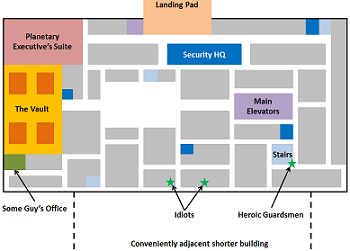
\includegraphics[width=\figwidth]{pics/18/25-large.png}
	\end{center}
\end{wrapfigure}
As we advanced Sciscitat finally got his shit together, and ordered us to ignore the battle (duh), avoid engaging any Cartel security forces (also duh), and to meet up with and assist the Interrogator. 
At his directions jogged down two halls and around a corner until we found ourselves in a window-lined hallway running the bank's entire south side. 
We kept our weapons ready, but thanks to advanced warning from the Inquisitor and Snitch, managed to dodge into side rooms and avoid two groups of Security troopers heading towards the battle. 
Once again, a few scribes saw us, but even covered in dried shit and carrying a psyker over one shoulder, Sarge's aura was enough to convince them that we were The Authorities and everything was under control.

Back when the shooting had first started, the Interrogator had found herself being very politely, but firmly escorted out of the gallery she'd been supposedly touring and into a shielded conference room. 
Her cover was still intact of course, but her unwanted protective detail refused to release her or budge without orders from the very distracted Security chief, leaving her somewhat trapped. 
She was sipping the rather decent tea that had been fetched for her and debating whether there was any way she could kill all five of her guards before one shot her, when there was a knock on the conference room's heavy wooden door. 
One of the guards flanking the door asked the other who it could be and reached for the door's handle, then it hit him.

\begin{wrapfigure}{O}{\figwidth}
	\begin{center}
		
\includegraphics[width=\figwidth]{pics/18/26.png}
	\end{center}
\end{wrapfigure}
Sarge's shoulder charge blew the door right off it's hinges, flattening the first guard under both it and Sarge's own considerable bulk. 
The second guard, who'd been standing on the other side of the door, was still staring in disbelief when Tink stepped through the opening and whapped in the stomach with his electrified wrench. 
The third guard was on the far-left side of the room and started to raise his autogun, only to drop it as Twitch's not-quite-expertly-thrown knife hit him in the eye handle-first. 
The fourth guard, who'd been in the process of pouring the Interrogator another cup of tea, flinched backwards with a choked shout as the scalding liquid he'd just poured was hurled back into his face. 
This all just left the final guard standing about a meter behind the Interrogator.

The Cartel security trooper, operating on automatic, brought his autogun to his shoulder and clicked off the safety. 
He began to draw a bead on Tink, who lacking any real cover, dove for the ground in a spineless attempt to put the Interrogator between himself and the imminent gunfire, while Twitch simultaneously started to draw his laspistol. 
Seeing that the demolitions trooper was going to be too slow, the Interrogator whistled a command at her rhinestone and pink bow covered cyber-mastiff, and then screamed as something flew over her head.

There was a ringing silence, broken only by the groans and whimpers of the disabled guards. 
The Interrogator rather shakily climbed to her feet, scanning the area for the jeweled comb that had been yanked from her hair. 
She paused at the sight of the half-crushed Guard behind her, and then turned to glare at Sarge.

>Who throws a door? 
Honestly.

\begin{wrapfigure}{O}{\figwidth}
	\begin{center}
		
\includegraphics[width=\figwidth]{pics/18/27.png}
	\end{center}
\end{wrapfigure}
So, the Breach and Clear went fairly smoothly. 
Especially considering that, due to Snitch's snitching, we were forced to do it "WITHOUT starting a gunfight with security and getting us in the exact same mess those other idiots are in, by the Emperor how do you even managed to breathe unassisted?" 

While we'd been at it, Doc and Snitch successfully kept several scribes and a curious janitor from getting close enough to make out anything but a few muffled thumps. 
Nubby, who was performing the same duty at the other end of the hallway had a bit more trouble when a pair of servant-types tried to get past him with a snack trolley for their "guest". 
The servants got a bit fussy when Nubby told them to bugger off but leave the snacks, especially when he started eating the hideously expensive dainties in front of them. 
Fortunately, before they got around to actually carrying out their threat to call the head of Security, the Interrogator and Snitch came over and were able to convince them all was well. 
The rest of us grabbed a few bites for ourselves as we passed, because hey, free snacks man.

The Interrogator led us at a brisk run to a maintenance closet, which turned out to be occupied by the Cleric, who'd gotten a bad electrical burn from somewhere and seemed to be grumpy with us for some unspecified reason. 
Doc helped him with his burn, while the Interrogator seized the bag of gear he'd been carrying and locked herself in the closet. 
We loitered around, watching the perimeter and trying to gauge how the other team's gunfight was going, and in a disturbingly short amount of time, the Interrogator re-emerged in full combat gear (though her cyber-mastiff still had its bows on). 
Without a word of explanation, she signalled us to follow, and broke into a run towards the western edge of the bank.

\begin{wrapfigure}{O}{\figwidth}
	\begin{center}
		
\includegraphics[width=\figwidth]{pics/18/28.png}
	\end{center}
\end{wrapfigure}
Based on the sound of things, we were trying to beat the other team to whatever the hell the objective was; 
once again, nobody was telling us anything. 
We just kept our weapons ready and raced through the corridors after the Interrogator and Cleric at a dead, well, jog since even our fitter teammates were a bit slow for our taste (lack of proper daily PT will do that to you). 
In any case, between the distraction being caused by the other team and our own's control over automatic doors, we managed to avoid getting bogged down and kept up a good pace until we reached our destination: 
some sort of big fancy office with two guards standing outside of it.

Both guards went down before they knew what hit them: 
one to a dart from the Interrogator's needlegun, the other more messily to her beribboned dog. 
She and the Cleric attempted to continue their charge into the office before anyone inside noticed us coming, only to run face-first into the door when it didn't automatically open. 
Sarge kept a straight face, but the rest of us snickered as we watched the rear and, since it seemed like the Inquisitor was losing control over the building's security systems, preemptively destroyed a pair of ceiling turrets Twitch spotted. 
After a bit of chatter with the boss about walls and fire and stuff, Tink was called up to plug his dataslate into the door controls, which did the trick.

The Interrogator and Cleric were through the door the second it unlocked, without even giving us a heads up, much less stopping to get our professional opinions on how to do it properly. 
It was only sheer bloody luck that the Cleric got hit in the shoulder instead of his face, and Sarge was half tempted to wait until the Interrogator had caught a bullet or three herself before he intervened. 
Good sense won out over spite though: 
a bit of covering fire and a grenade later, the Security guards were down and Interrogator's cyber-mastif dragged a whimpering senior banker out from under his desk.

\begin{wrapfigure}{O}{\figwidth}
	\begin{center}
		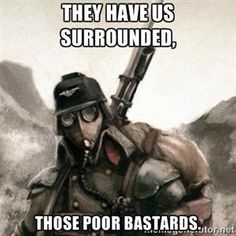
\includegraphics[width=\figwidth]{pics/18/29.png}
	\end{center}
\end{wrapfigure}
While the Interrogator interrogated, barking questions about vaults, codes, and artifacts at the terrified banker, we kept an eye on the door and lounged around the front office. 
Doc gave the Cleric a quick once over, choosing to just throw a bandage on the man's shoulder instead of trying to dig out the autogun round lodged in it. 
Those of us not on door duty established that the security guards hadn't been carrying any salvageable munitions, and had moved on to checking the banker's office for "important clues" (see: 
snacks and/or a minibar), when Snitch finally caught up. 
Upon arrival the huffing and puffing psyker, who was probably regretting his decision not to let Sarge carry him again, was called up to assist with the questioning, while we were told to get out and "go secure the perimeter or something". 
We found that order to our liking.

On the list of desperate and heroic Imperial Guard defensive actions, this wasn't one. 
I mean, theoretically the Cartel must have had some real crack troops, they were a sector-wide shipping conglomerate after all, and just holding their sub-spire against the local underworld must've taken at least a few competent troopers. 
Those guys must've been busy somewhere else though, possibly fighting the other team, because the Security troopers that got sent our way were even more pathetic than raw Guard conscripts given the lack of Commissars to stiffen their resolve. 
Might've been a different story if all those automated sentry turrets had been working, but since two separate Inquisition teams had infiltrated their systems, someone was probably really regretting skimping on their troops' training budget.

\begin{wrapfigure}{O}{\figwidth}
	\begin{center}
		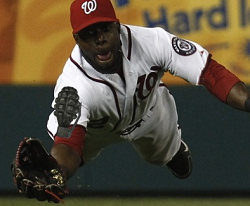
\includegraphics[width=\figwidth]{pics/18/30.png}
	\end{center}
\end{wrapfigure}
The first Cartel Security patrol sent to rescue the Banker came in along the windowed corridor, ran into a pair of anti-personnel mines, and abruptly decided they had better things to do than find out if there were any more. 
Sarge popped a few shots over their retreating heads to really drive the point home, and then just left the hallway unwatched in favor of helping Twitch secure the one leading towards the battle with the hostile team.

Doc and Nubby nearly ran into a second security patrol while trying to figure out that most important part of any good perimeter: 
a good escape route. 
The two of them had been inspecting a small stairwell that went down five or so levels, when a bunch of Security troopers piled in through one of the lower doors. 
A few reflexive shots were traded, none of them doing any real damage, just encouraging everyone to get behind some cover, and then Doc got the bright idea to try and convince them that we were PDF reinforcements. 
The troopers actually bought this, but despite their apparently room-temperature IQs, Doc was having some trouble convincing them not to come up the stairs. 
Nubby rolled his eyes, grabbed the pair's last frag nade off Doc's belt, and informed the Security troopers that he was just going to toss down a copy of our "orders". 
Doc glared at Nubby, but helped him keep the survivors pinned down until Tink showed up to seal the stairway door.

\begin{wrapfigure}{O}{\figwidth}
	\begin{center}
		
\includegraphics[width=\figwidth]{pics/18/31.png}
	\end{center}
\end{wrapfigure}
The Inquisitor hadn't managed to close all the work-area doors in the quadrant before he'd been kicked out of the security system, so Tink (with the grudging assistance of the tech-priest) used his dataslate to seal the ones he missed. 
The tech-priest was not informed that step-two of this process involved frying the closed doors' controls. 
After assisting Doc and Nubby, Tink was working his way down the last section of offices, near where Sarge and Twitch were building their big barricade, when he noticed something on his map and paused to scan the cubicle-filled office area with his goggles. 
He commed Sarge and asked, just hypothetically, if it'd be worth knocking down a few flimsy walls and giving the hostile team a little surprise right as they reached their destination.

It really was just too good an opportunity to pass up. 
A few minutes later, during which the big barricade was finished and a rather dubious escape route was planned out, all of us were gathered in a cubicle a few meters away from the door leading to the other team's supposedly-secure left flank. 
Twitch had just put the finishing touches on the nice fat satchel charge that would be our opener, when the Inquisitor commed us and demanded he and Tink immediately return to the Banker's office. 
Sarge asked if it could wait, since we were about to sort out the whole "hostile Inquisition team trying to beat us to the objective" problem. 
What we expected was grudging acceptance and a bit of yelling about not informing him of our plans; 
what we got was an enraged scream of an order to pull back IMMEDIATELY.

Sarge tried to placate Sciscitat, explaining that whatever it was he needed doing, it could probably wait until the other team was dead. 
The Inquisitor didn't respond too well to this, just repeatedly screaming "NO" while (judging by the sound) slamming his keyboard against his desk. 
Sarge's attempts to get an explanation for this odd behavior were interrupted by someone opening the door. 


\begin{wrapfigure}{O}{\figwidth}
	\begin{center}
		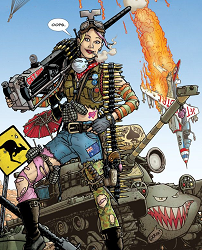
\includegraphics[width=\figwidth]{pics/18/32.png}
	\end{center}
\end{wrapfigure}
Since we'd just received fairly explicit (if a bit unhinged-sounding) orders not to engage, we didn't open fire on the enemy agent who came through the door; 
unfortunately that didn't stop them from shooting at us. 
The familiar mohawk-sporting Ganger girl, who'd probably overheard Sarge arguing with the Inquisitor during a lull in the firefight, noticed Doc before he ducked out of sight and with a shout of "NOT YOU ASSHOLES AGAIN" opened up with her heavy stubber.

Fight not being an allowed option, we settled for flight. 
The fiberboard and fabric walls didn't do much to stop the Ganger's stub rounds, but they did at least break her line of sight, so after the first burst (which left two rounds embedded in Doc's backplate and Twitch with a bleeding arm) she was pretty much just spraying the room at random. 
We kept low, trying to keep as many desks, cogitators, and scribes as possible between us and her while we worked back towards where we'd cut our way in. 
Nubby, who was valiantly leading the retreat, had just reached the exit when the Ganger abruptly stopped firing and shouted "but it's the guys who shot me in the ass!" at someone out in the hallway, who replied with an almost Sarge-like bellow of "THEY'RE ON OUR SIDE YOU IDIOT".

Doc, in what definitely wasn't his smartest moment, peeked over a cubicle and asked "We are?", but the Ganger was too busy staring incredulously at the man out in the hallway to shoot him. 
Twitch told him it was obviously a trick and to get back down, while Tink and Nubby just shrugged at each other. 
Sarge sighed and silently cursed all Inquisitors as Sciscitat, who'd disconnected his comm channel when the shooting started, came back online to tell us the other team was no longer considered hostile, and we were all to pull back to the Banker's office before any more idiocy occurred.

On the bright side, at least this time we figured it out BEFORE exploding half of the other team. 
So, ya know, progress.

\begin{wrapfigure}{O}{\figwidth}
	\begin{center}
		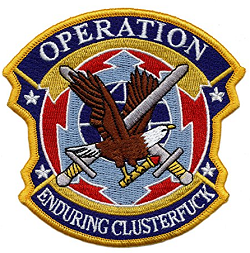
\includegraphics[width=\figwidth]{pics/18/33.png}
	\end{center}
\end{wrapfigure}
Honestly, at this point we just gave up trying to understand the overall strategic situation; 
it was just such a colossal mess and it seemed like we were getting more intel from the guys we'd been shooting at than our own teammates. 
The important thing was the other team was friendly and running interference for us while we looted the thing from the vault, and we needed to get moving right now to help with that, because a dozen fliers full of enemy reinforcements had just landed. 
Also, our teammates were in the vault now (somehow), Face and the Assassin were chasing someone on the roof, Snitch needed to do something, the tech-priest was seeing odd power readings, the Cleric had gotten shot (again), and the Inquisitor was going to flay us alive if we didn't get moving RIGHT NOW.

We got back to the office to find it empty except for a now-comatose Banker and a previously hidden passage leading into the vault. 
The place turned out to be even larger than expected, with thousands of lockboxes lining the walls and a dozen sub-vaults scattered around the room. 
To all of our disappointment (especially Nubby's) there were no loose piles of easily-pocketable cash, gold, or jewels lying around, just a bunch of dead Cartel security guards, a few potted plants, and a dug-in squad of those Secret Police guys trading fire with our teammates. 
Sarge reported our arrival and went off with Doc and Nubby to sort out that mess, and sent Tink and Twitch do whatever super important thing the Inquisitor had wanted them for.

\begin{wrapfigure}{O}{\figwidth}
	\begin{center}
		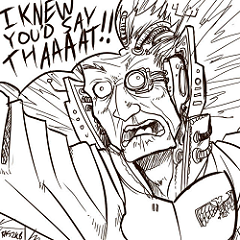
\includegraphics[width=\figwidth]{pics/18/34.png}
	\end{center}
\end{wrapfigure}
At Scisciat's order, Twitch and Tink followed the Interrogator from cover to cover across the room to one of the sub-vaults, where Snitch had his forehead pressed against the door and was starting to glow. 
The two guardsmen, who both had far more experience in the perils of warp use than anyone wants, abruptly decided there was too much incoming fire for them to push forward yet. 
They watched in smug satisfaction when, after all of three seconds, Snitch started convulsing and the Interrogator fell to her knees clutching her head and screaming while her dog lunged and snapped at invisible enemies. 
Twitch asked Tink whether they should shoot the psyker if his fit lasted for more than a minute, but fortunately the warp-ghosts or whatever dissipated before they reached a decision.

To our considerable surprise, Tink and Twitch weren't ordered to open the vault and collect whatever weird shit was in it. 
After Snitch and the Interrogator had recovered enough to report their findings, Sciscitat told the two troopers to destroy the vault's contents and ordered the entire team to prepare to pull out the second the charges were set. 
These wonderful orders were slightly marred by the way he went on to try and explain the best way to do said demolition to us, but he eventually accepted that Tink and Twitch did indeed know how to melt a hole and stick a bomb in it.

Three minutes, two plasma power-packs, and a very delicate insertion of a high explosives through a still-glowing hole later, the bomb was set. 
Sarge reluctantly used his last grenade to take care of the one Secret Police agent who kept refusing to die, picked up Snitch, and led the withdrawal. 
Our group paused in the Banker's office, waiting while Sciscitat yelled at various other people and then started a countdown to "Phase 19". 
He'd only reached eleven when the entire building shook, the lights flickered, and then every cogitator, appliance, and lighting fixture in the bank exploded.

\begin{wrapfigure}{O}{\figwidth}
	\begin{center}
		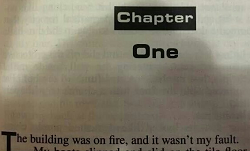
\includegraphics[width=\figwidth]{pics/18/35.png}
	\end{center}
\end{wrapfigure}
Over the next few seconds we realised three things. 
Firstly, our long range comms were down, cutting us off from the Inquisitor and most of the rest of the team. 
This bothered the Interrogator and Cleric a lot more than us. 
Secondly, that hadn't been Twitch's bomb. 
The demolitions trooper looked at his detonator in confusion for a few seconds before hesitantly clicking it, triggering a much smaller and closer explosion, followed by a burst of painful psychic wailing which sent Snitch into convulsions. 
Twitch nodded in satisfaction and looked at Tink, who after a few seconds of blank staring, excitedly declared that it must've been the power station overloading. 
Finally, the entire bank was on fire and the water in its sprinklers had probably been sitting stagnant for the better part of three hundred years. 
As our teammates, the Interrogator especially, swore and gagged, Doc pointed out that we'd become disturbingly used to these smells. 
Sarge nodded, clicked his combead a few times to check if it was going to spontaneously start working, and then announced that it was time to make like a tree and jump out of a burning building.

Back before we'd left the van there'd been a discussion about how much gear to bring, aside from a full combat load and our entire limited supply of explosives of course. 
Twitch had insisted that he wasn't going up in any up-spire deathtrap without a way to get down, which is why he'd be bringing his grav-chute. 
Tink had chimed in, assuring the rest of us that the chutes were much less bulky now that he'd removed the extra bits (like all the safety features and backups). 
The two of them had been pretty smug when, after verifying there weren't any less insane options, Doc and Nubby had proposed just jumping out the window as a possible escape route. 
Of course, that decision had been based on the theory that we'd be alone, but Tink said he was almost positive the chutes could take a little extra weight.

\begin{wrapfigure}{O}{\figwidth}
	\begin{center}
		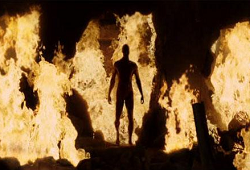
\includegraphics[width=\figwidth]{pics/18/36.png}
	\end{center}
\end{wrapfigure}
Snitch wasn't conscious enough to object, but the Cleric and Interrogator were not very happy about being carried down the first five story drop, and there was the stupidest argument about bringing the damn cybernetic murder-dog. 
Complaints aside though, everyone got down to the adjacent roof just fine, even Doc who had to do it on only one grav-coil on account of the stub round lodged in his left one. 
From that landing it was just a short run to the next jump with decent cover the whole way. 
Not that any of the Cartel security forces seemed interested in taking shots at us: 
they were a bit preoccupied with fleeing the Bank, as well as several other nearby buildings that must have been hooked to that power station too. 
Even the Secret Police fliers were taking off, possibly because the Bank seemed to be listing slightly to the left now.

Two more drops got us down to where we could see the alley that we'd parked the vans in. 
It was Nubby who got the edge first; 
the little trooper peeked over, and after a pause, asked Tink whether our vehicle had been hooked up that power grid thingy. 
Tink said no, and Nubby suggested it must be on fire for a completely unrelated reason then. 
We all ran over to verify that, yes our un-trusty steed was on fire. 
Everyone simultaneously looked at Twitch, who muttered something about anti-theft measures. 
After a few seconds of pondering this and the fire below, Doc raised the question of who in their right mind would try to steal such a shitty van, and then trailed off. 
There was an ugly, congealing silence broken only by our teammates asking what was going on and an increasingly loud thumping from the flaming van. 
We watched in horror as the van's rear door broke open with a bang and tall figure in  stepped out of the flames, burning scraps of duct-tape dropping off blackened armor like thematically appropriate snowflakes. 


Twitch informed everyone present that he'd told us so.

\begin{wrapfigure}{O}{\figwidth}
	\begin{center}
		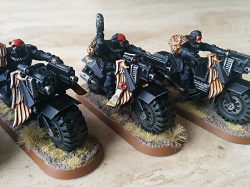
\includegraphics[width=\figwidth]{pics/18/37.png}
	\end{center}
\end{wrapfigure}
We wanted to just shoot the guy, we really, REALLY wanted to. 
If Aimy had been there to guarantee us a kill shot we might've gone for it. 
As it stood though, it was just too much of a stupid risk to be worth it. 


It wasn't that we were in hostile territory, cut off from our superior and half our teammates, and watching our escape vehicle burn to the ground in front of us. 
Or at least not just that. 
As the Traffic Officer stepped out of the van, he waved a badge we hadn't seen before in the air. 
Several specks circling in the smoke above the sub-spire descended and resolved into an entire platoon of jet-bike riding Arbites who, despite the fact that he was wearing a traffic cop's uniform, began following the man's bellowed orders to lock down the entire street. 
At the back of the alley, the scan-van started to pull out only to stop and return to its spot as two jet-bikes blocked the exit. 
After a few seconds the tech-priest got out, shot a glare in our direction, and disappeared through a small maintenance hatch before the Arbites started rounding up pedestrians.

Escaping from the sub-spire proved to be more embarrassing than anything else. 
The initial debate over what to do had involved a lot of totally unjustified criticisms from the Interrogator and Cleric, and possibly few harmless threats of roof-throwing from some of us, but before things escalated Snitch woke up and announced Face was calling him. 
The psyker and assassin turned up in their little fliers, and while they didn't have nearly enough room to fit us all, at least they got our teammates out of our hair. 
The fliers also had long range comms, which put us back in contact with Sciscitat, who was very busy with other things and wanted us to hold position for "six to fourteen hours". 
Sarge told him and the rest of the team where to shove it, and announced our intention to get out on foot.

\begin{wrapfigure}{O}{\figwidth}
	\begin{center}
		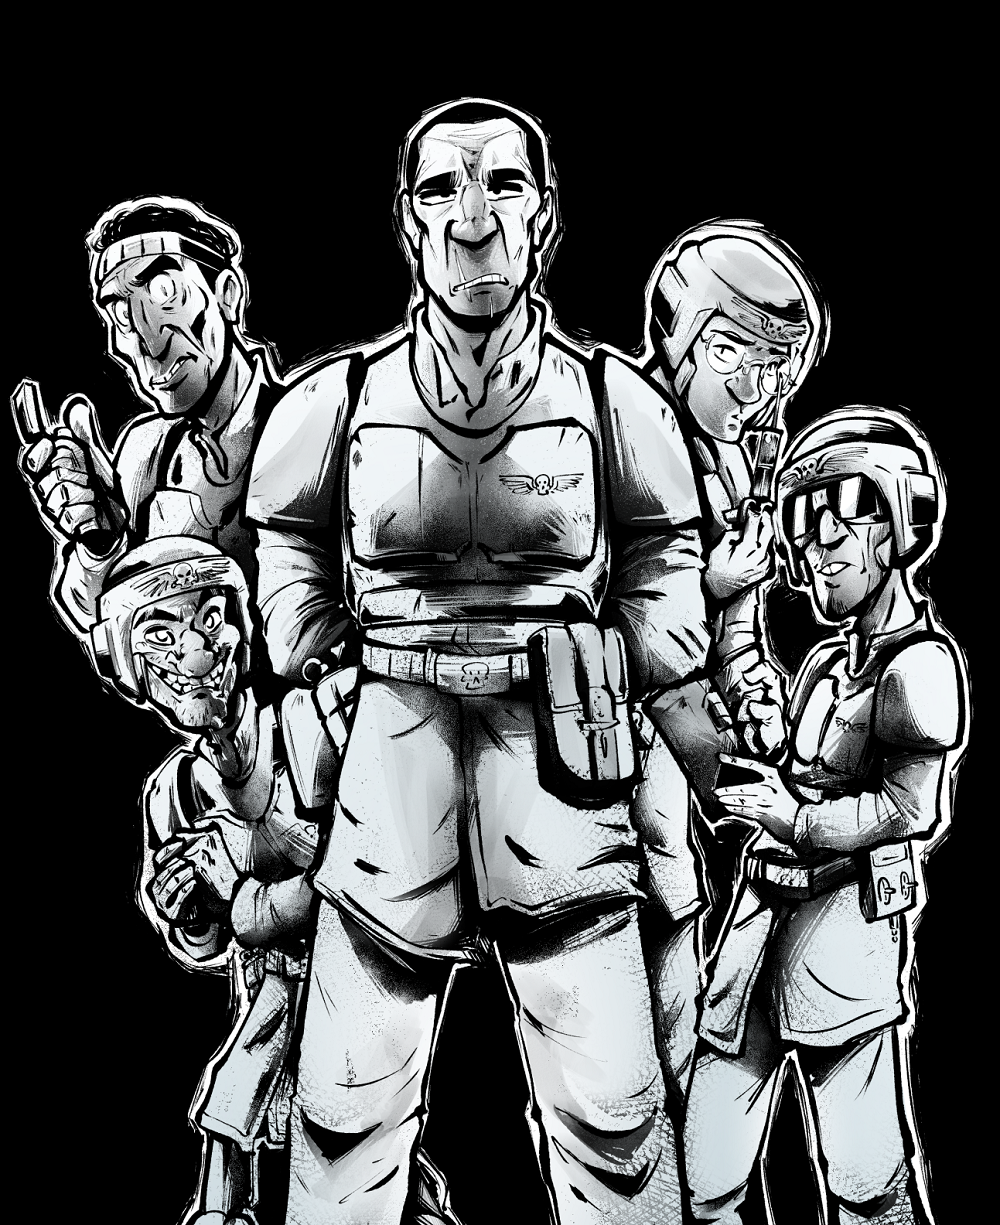
\includegraphics[width=\figwidth]{pics/18/38 large.png}
	\end{center}
\end{wrapfigure}
The Inquisitor had objected of course, as had his toadies, insisting that there was no way we'd get past any of the security checkpoints. 
Sarge's suggestion that we join up with the tech-priest hadn't worked, since the cogboy wasn't in comm contact, and we were told that any attempt to grav-chute off the sub-spire would get us shot down by Cartel security fliers. 
There was a bit more arguing, and then Doc raised the question of how the OTHER team had extracted. 
A short run back into the burning (and now obviously tilting) bank and a bit of grav-chuting down that big stairwell later, we caught sight of a familiar pink mohawk and Sarge nearly got his head shot off as he tried to land in the middle of a trio of incredibly twitchy Inquisition agents.

Of the group, the only one we'd seen before was the Ganger, though we recognized the voice of a grizzled older man in power armor as the one who'd yelled at her. 
The third agent was a longcoat and wide-brimmed hat wearing man with some sort of fringe-world accent, who seemed to be the least offended by our impressive collection of smells. 
They gave us some very dubious looks when we asked about catching a ride, and the Ganger made a few pointed comments about people who shot other people in the ass expecting favors. 
Sarge, who'd entirely ran out of fucks to give, told her to shut up and look on the bright side, since he'd been originally aiming for her in the head before Sciscitat decided he wanted a prisoner. 
This won a laugh from the fringe-worlder and caught the attention of the armored man, who demanded to know if Sciscitat was really commanding the operation in person. 
Sarge tried to go poker faced, but relented when Nubby cheerfully informed them that "Quisitor Asshat" was sitting up in orbit on his comfy spaceship. 
As Tink and Twitch chimed in with their own opinions of our commanding officer and teammates, Sarge saluted the ghost of operational security; 
Doc assured him it was probably for the best.

\begin{wrapfigure}{O}{\figwidth}
	\begin{center}
		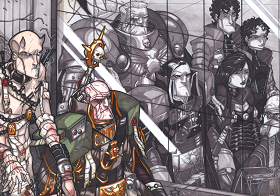
\includegraphics[width=\figwidth]{pics/18/39.png}
	\end{center}
\end{wrapfigure}
We spent most of the uneventful hike out through the maintenance tunnels talking with our new friends. 
Sadly the old armored guy (who turned out to be yet another Interrogator) wasn't that talkative, and the limping Ganger mostly just swore and glared at us, even after grudgingly accepting some drugs from Doc. 
The fringe-worlder, on the other hand, seemed happy to tell us as much as his boss would let him, and over the following two hours he painted us quite a picture. 
Admittedly it was conveyed in a nigh-incomprehensible drawling accent interspersed with far too many "quaint" sayings about his granpappy's ol' grox, but it was still more than we'd gotten from our own team.

The gist of it was that everything was a complete clusterfuck. 
Basically, when the Conspiracy had made their move on Oak, they'd stolen several eldritch artifacts from one of his little facilities. 
The artifacts had been taken to the Conspiracy's base here on Haarlock's Wager, which we knew about because one of Oak's allies had followed their ship. 
Unfortunately, instead of waiting for backup like a sane person, this Inquisitor had just gone in guns blazing, which is why this was our problem now. 
To the guy's credit though, it was also why the planet's third moon had a shiny new metal-rich asteroid belt around it instead of a top-secret orbital facility and only one traitorous Inquisitor in the system instead of four. 


Unfortunately that last traitorous Inquisitor had proved to be a bit a problem. 
According to the fringe-worlder she was just a junior member of the Conspiracy who'd actually arrived in system after the attack had lready started, but she turned out to be a powerful Sorceress with a pet Demonhost, which she'd sicced on the Inquisitor's vessel while he was busy. 
The end result was our guy being trapped on a hostile planet, desperately trying to hide the artifacts and get word out before he was torn apart by an enraged daemonhost. 
He was only moderately successful.

\begin{wrapfigure}{O}{\figwidth}
	\begin{center}
		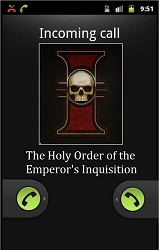
\includegraphics[width=\figwidth]{pics/18/40.png}
	\end{center}
\end{wrapfigure}
Where the fringe-worlder and his teammates came into this was about a week later, when one of these messages reached their Inquisitor (counting ours this made him the SEVENTH one involved in this mess). 
Now, according to our narrator, his Inquisitor wasn't actually one of Oak's allies. 
In fact, he apparently held a pretty deep grudge against the man and everyone associated with him on account of how one of Oak's little training missions had stumbled into the middle of a decade-long investigation of his and blown the whole thing out of the water (we checked, it wasn't us). 
Despite not liking Oak, and not having ever heard of the Conspiracy before either, whatever had been in that message had been enough to get the fringe-worlder's boss on board. 


So this new Inquisitor and his team had touched down about a week ahead of us to find the first guy dead, and the Sorceress tearing the entire hive-world apart in a desperate search for the artifacts. 
From there it had been a sort of competitive scavenger hunt, with the fringe-worlder's team having the advantage of a big dead-drop full of clues and directions, while the Sorceress had the aid of the entire planetary government. 
Well, partial aid: 
it'd been her now-dead Conspiracy bosses who'd had the planet under their thumbs and a lot of that power had died with them. 
The Sorceress was apparently some sort of master manipulator though, and she was steadily regaining control. 
In any case, the team had snagged one artifact with no problems, had been beat to another by the Sorceress, and had been in the process of claiming the third artifact from the Cartel when everything hit the fan.

\begin{wrapfigure}{O}{\figwidth}
	\begin{center}
		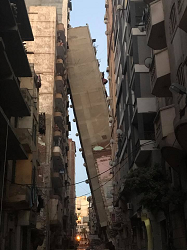
\includegraphics[width=\figwidth]{pics/18/41.png}
	\end{center}
\end{wrapfigure}
Interestingly, nobody present (aside from the Ganger) held us to blame for the deal with the Cartel going south. 
They'd already been prepping in case that notoriously mercenary institution turned on them, hence their sabotage team in the basement and all the heavy weapons they'd brought to the Bank, but the hand-off had actually been going smoothly right up to the point where the Sorceress had landed on the roof. 
A short chat between her and the Cartel's Planetary Executive Officer later, Security was trying (very unsuccessfully) to kill them.

At this point we had to supply some of our own details, explaining that our team had actually been trying to beat them to the prize, and all the confusion with us misidentifying them. 
The fringe-worlder reciprocated with the story of how their Inquisitor had nearly run into Face and our Assassin while all of them tried (and failed) to kill the Sorceress before she escaped in the PEO's armored flier. 
The rest we all pretty much knew: 
everyone started working together, Sciscitat was tasked with grabbing the artifact, but had us destroy it instead for some reason, and both teams were able to make a mostly-clean escape thanks to the "spontaneous" explosion of the power station under the Bank. 
Nobody had even died: 
most of the other team (including the tech-priest and Sister we'd shot up) had extracted via a disguised flier, while the three walking with us had pulled out on foot after getting cut off from the LZ. 


So really, when you looked at things objectively, it had been a pretty successful mission. 
Sure, a few people had gotten shot (three times in the Cleric's case), the Arbites might've impounded our vehicles, and we'd heard some very building-collapsy sounds somewhere above us on our walk. 
Oh, and we'd destroyed the artifact instead of stealing it, but that had been Sciscitat's idea, not ours… Still though, not a COMPLETE failure right?

For some reason we didn't feel like the Inquisitors would agree with us.

\begin{wrapfigure}{O}{\figwidth}
	\begin{center}
		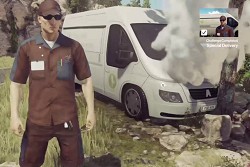
\includegraphics[width=\figwidth]{pics/18/42.png}
	\end{center}
\end{wrapfigure}
Actually, one of the two Inquisitors proved to be surprisingly reasonable about the whole thing, it just wasn't ours. 
We met the second team's Inquisitor as we finally climbed out of the maintenance tunnels a good two kilometers away from the Cartel's sub-spire. 
We exited into a disreputable looking garage, which was populated by a bunch of biker types (who could've easily been the Ganger's siblings) as well as a tired-looking truck driver and his vehicle. 
While our companions paid off the bikers, the truck driver took in our filth-encrusted appearances and announced that we would be riding the back. 
This led to a bit of difficulty when the truck's cargo area turned out to be half-full of the exact sort of boxes and metal drums that Orks hide in to ambush unsuspecting guardsmen, at least according to Twitch that is. 
This in itself wasn't a problem, we were perfectly willing to check the boxes for kommandos/loot before boarding, the issues was the way the driver assured us his cargo was ork-free BEFORE any of us had mentioned them. 
Twitch noticed this and reacted about as well as you'd expect.

Fortunately, the Inquisitor (as he was introduced to us after things had calmed down) had just as good a reaction time as Twitch, and enough telekinetic skill to jerk three successive weapons out of the demolitions trooper's grip. 
Even more fortunately, he proved to be a good sport about the whole thing; 
he even gave Twitch back his guns and let us inspect the truck's contents (no Orks, but nothing worth pocketing either sadly) before personally driving us back to our base.

\begin{wrapfigure}{O}{\figwidth}
	\begin{center}
		
\includegraphics[width=\figwidth]{pics/18/43.png}
	\end{center}
\end{wrapfigure}
We didn't get to see the meeting between the two Inquisitors; 
in fact, we weren't even allowed into the base. 
Our teammates at the door, the Interrogator especially, acted like it'd been OUR idea to spend half a day tromping around in the sewers and refused to let us in until we'd visited the shallow pool of chemical-laden water that the locals referred to as a "lake". 
At least all the acid meant we didn't need to bother with soap... 
or scrubbing… Tink recommended that we clean our weapons and more delicate equipment somewhere else. 
Anyway, by the time we were finally readmitted to our own damn base the other team and their Inquisitor had left, leaving us without any handy distractions when Sciscitat had us step into the secure conference room for our debriefing.

Honestly, it didn't go as bad as we'd expected, partially because Sciscitat too distracted with something else to properly chew us out, but mostly because Snitch wasn't there to rat us out as we creatively shifted blame onto various other parties (mostly the other team and the tech-priest). 
Still though, there was a lot of yelling about insubordination, stupidity, Arbites, and sharing intel with the other team. 
He seemed especially peeved at us for bringing that other Inquisitor to our secret base, which was a little unfair since we hadn't said a word about it. 
I mean, he was a psyker, what were we supposed to do? 
Shoot him before he read our minds? 
We did point out that Twitch had actually tried to do that, but that only got us yelled at more. 
Eventually though, Sciscitat got tired of yelling at us and getting monosyllabic responses, and ordered us back out to our quarters, where we were to "Just stay out of the way and try not to unsuccessfully kidnap any more interplanetaraly famous Arbites."

\begin{wrapfigure}{O}{\figwidth}
	\begin{center}
		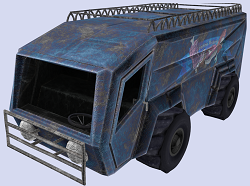
\includegraphics[width=\figwidth]{pics/18/44.png}
	\end{center}
\end{wrapfigure}
The days that followed were filled with tireless Inquisitorial investigation as both our team and the other worked to decode the location of the next artifact before the Sorceress. 
At least we were pretty sure that's what everyone was doing, our involvement primarily consisted of watching the base while everyone else was out and playing poker in our quarters when they weren't. 
This suited us fine: 
we were busy enough between dealing unpleasant side effects of the Munitorum-grade antibiotics Doc forced on us and taking as many showers as possible.

Despite our non-involvement we did pick up a few scraps of information. 
For instance, we found out the scan-van was somehow recovered from Arbites custody after only a day, as (to our disbelief and dismay) was our shitty van. 
How it survived was a mystery; 
Twitch was especially up in arms, insisting that his anti-theft device should've burned out every scrap of electronics and left the engine beyond repair. 
Despite that though, it rolled into our garage as barely-functional as ever, with only scorch marks and a half-melted pair of seats to testify to its immolation. 
We weren't sure whether to blame the tech-priest or Sciscitat for this, so we just settled for hating them both. 


On the note of the vans, Sarge was called into a short briefing on the subject of the Traffic Officer, where he learned that the man had been reinstated as some variety of Judge in the Jack Hive Arbites. 
There was a bunch of political stuff involved too, something about the Arbites being pissed at the planetary government, the important part was the Officer was now leading an investigation into what had happened at the Cartel's sub-spire. 
This was technically good news, since a big investigation would cause more problems for our enemies than us, but was counteracted by the descriptions of five "rogue PDF stormtroopers" that had been given to every Arbite and traffic cop in the hive. 
Our orders to stay inside were reiterated.

\begin{wrapfigure}{O}{\figwidth}
	\begin{center}
		
\includegraphics[width=\figwidth]{pics/18/45.png}
	\end{center}
\end{wrapfigure}
By the end of the week Doc had gotten all of us, including those of our teammates who'd gotten themselves shot, back into fighting shape. 
The one exception to this was Snitch, who'd developed some sort of irrational nausea around Doc, and kept spewing everywhere until the medic gave up and let someone else try treating the psyker's minor injuries and infections. 
Tink meanwhile, had repaired Doc's grav-chute despite the medic's protests against ever using the damn thing again. 
He also made a few more attempts to fine-tune his uncooperative plasma weapon, but got yelled at when he tried to test it inside the base. 
Twitch and Nubby, through a dedicated campaign of whining, dark comments about what Twitch might build himself, and threats to go to the other team, managed to convince Sciscitat to refill our limited supply of explosives. 
Nubby then went to the other team anyway, but only managed to score a handful of nades off the Ganger before her boss yelled at her for trafficking on Inquisition time and stopped bringing her to our base for meetings. 
Sarge just kept an eye on the rest of us and enforced that not-leaving-the-base rule until the next artifact was found.

Our first clue that progress had been made was our entire team returning in the middle of the night and rushing into the communications room. 
The second was when the other Inquisitor showed up at our hab unit's front door with half his posse and informed Sarge that he would level the entire hab-block if we tried to go get the artifact without him. 
Sarge, not being paid enough to deal with this sort of Inquisitorial power-politics bullshit, just showed them all into the comm room. 
Ignoring the massive amount of stink-eye directed towards him by our teammates for doing this, Sarge invited the rest of us in to help keep an eye on the dangerous people we'd just let into the base (really though, it was just so we'd all be there to protest if they tried to send us into the sewers again).

\begin{wrapfigure}{O}{\figwidth}
	\begin{center}
		
\includegraphics[width=\figwidth]{pics/18/46.png}
	\end{center}
\end{wrapfigure}
Sciscitat's usual self-praise-filled briefing style was hampered somewhat by the presence of the other Inquisitor, who had a tendency to make pointed sarcastic remarks about who'd actually done what work. 
We decided we liked the man, psyker or not. 
Anyway, skipping over all the barbed comments, unasked-for critiques, and other such low-level conversational sniping, the briefing started with a picture of a rune-covered box with a skull for a latch, whether this was the artifact itself or if it was actually inside the box was not explained to us. 
Sciscitat claimed the box had been given to a small local courier service by the now-dead Inquisitor, but instead of being quietly hidden away as he'd ordered, it'd wound up in the hands of the biggest underhive Crime Lord in neighboring Queen Hive. 


The artifact falling into the hands of the local underworld wasn't really that unexpected, in fact the dead Inquisitor had mentioned the possibility in his notes, the odd part was what the Crime Lord had decided to do with it. 
Instead of immediately fencing the artifact, or hoarding it away until the heat died down, this guy decided the best thing to do with this evil spooky box thing was to use it as the grand prize for some sort of high-stakes eldritch artifact poker tournament. 
Seriously. 


Needless to say, everyone was a little bit dubious; 
even Sciscitat, who was the one presenting the evidence, kept pausing to re-read his notes and rhetorically ask WHY. 
This wasn't even some megalomaniacal rogue trader or spoiled planetary noble, by all accounts the Crime Lord was a shrewd, level-headed, hardworking businessman with only a minor tendency towards throwing rivals into vats of boiling toxic waste. 
It really made no sense, and the other team's Inquisitor kept insisting that it must be some sort of trap, but eventually he became resigned to fact the he lived in a universe where common sense no longer existed. 
We welcomed him to the club. 


\begin{wrapfigure}{O}{\figwidth}
	\begin{center}
		
\includegraphics[width=\figwidth]{pics/18/47.png}
	\end{center}
\end{wrapfigure}
The other Inquisitor, perhaps still feeling a bit unhinged from his change in worldview, announced that our only option was to enter the poker tournament ourselves. 
Surprisingly, Face immediately seconded this, volunteering to be the one to enter, and even more surprisingly, so did the Assassin, who proposed using the one artifact the second team had recovered themselves as our ante. 
The idea began picking up speed at an alarming rate, with several of our theoretically sane teammates, as well as Tink and Nubby, excitedly offering suggestions. 
The rest of us had enough experience with bad ideas to recognize a truly terrible one in the making, and watched with growing unease.

Doc made some futile attempts to politely interject some sanity into the conversation, while Twitch just muttered to himself about psykers making everyone suicidal tightened his lead-foil lined helmet. 
Sarge was steeling himself for a more-yelly attempt than Doc's, but was beaten to it as Sciscitat blew his hologram up to maximum size and volume, and loudly demanded to know whether everyone had lost their minds. 
We deeply appreciated the ensuing lecture on why we would NOT be entering a high profile poker tournament guaranteed to be attended by our enemies, or risk the single artifact in our possession in said tournament, or count on some sort card-reading of x-ray eyepatch to guarantee us victory. 
Admittedly, we could've done without him using us as a reference point for the relative stupidity of an idea, but whatever.

As Sciscitat wound down everyone looked a bit sheepish; 
especially the other team's Inquisitor, who kept shaking his head and quietly asking himself what he'd been thinking. 
They all perked back up before long though, and by the end of the briefing had hacked out a "far simpler" twenty-seven stage plan to sneak in and steal the evil box thing while tournament was in process. 
Thankfully our part was going to be nice, simple, and almost certainly sewage-free.

\begin{wrapfigure}{O}{\figwidth}
	\begin{center}
		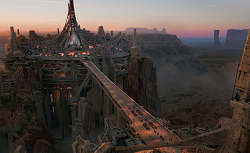
\includegraphics[width=\figwidth]{pics/18/48.png}
	\end{center}
\end{wrapfigure}
While two teams of highly trained Inquisitorial agents infiltrated the spiretop fortress-mansion of a slightly megalomaniacal Crime Lord, we were assigned the arduous task of making sure nobody stole our vans. 
It was a tricky job, that entailed a lot of very difficult napping, card-playing, smoking, and fast-food eating, but someone had to do it.

The Crime Lord's mansion was on its own little spire only a few hundred meters above the Queen Hive's smog clouds, and had only two major entrances. 
One was a big gaudy landing pad flanked by disguised anti-air batteries, where a steady stream of incredibly rich people were landing their flying vehicles and making their way into the mansion's main level. 
The other was a small utilitarian retractable causeway on the far side of the mansion; 
for service vehicles and all those non-rich people who were regretfully necessary for keeping things running. 
Guess which one we got to stake out.

While the scan-van positioned itself to have a good view of the landing pad, our shitty van and a pair of far-better quality unmarked getaway vehicles were parked in the large parking garage that served as a sort of waiting area for the causeway. 
As it turned out, our guarding of the vans was actually pretty necessary, since apparently the Crime Lord's normal business had all been put on hold until his insane poker tournament was over. 
We found ourselves rubbing elbows with a wide variety of terminally-bored people, ranging from underhive gangers, to mid-hive businessmen, to a bunch of off-planet mercs with a very unhappy-looking man tied up in the back of their vehicle. 
Between our unmarked, but obviously guard-issue gear, and our own palpable aura of slightly-paranoid boredom, we fit right in as we settled down to wait for our teammates to get on with the mission.

\begin{wrapfigure}{O}{\figwidth}
	\begin{center}
		
\includegraphics[width=\figwidth]{pics/18/49.png}
	\end{center}
\end{wrapfigure}
For lack of anything better to do (and because we'd been ordered to) we kept an eye on the vehicles going over the causeway. 
Not that anybody actually expected anything important to come in that way: 
the Inquisitors had intel that the Sorceress would be attending the tournament and had distributed some pictures of her to us, but she'd obviously be landing up at the pad with all the rich people. 
The most anyone expected were some reinforcements if the Crime Lord discovered our infiltration, or possibly a few APCs of Secret Police if the Sorceress decided to take a more direct approach, both of which would be dead obvious. 
Since Twitch tended to watch hard enough for a dozen people, he was put in charge of this while the rest of us kicked up our feet and made the best of our first excursion outside the base in over a week.

Over the course of about three hours of idling Twitch managed to spot a dozen "suspicious" catering vehicles, Sarge punched out a ganger who seemed too interested in one of the getaway-cars, Tink and Doc learned never to buy a "genuine meat product" Sausage-inna-Bun from a street vendor, and Nubby got told that while spitting over the edge at passing vehicles was almost acceptable, hucking beer bottles at them definitely wasn't. 
Deprived of his entertainment, our self-appointed quartermaster wandered off for a while and met various Guys who he proceeded to get to Know; 
he returned a bit later to tell the rest of us that he was a little short. 


Once we were done laughing, Nubby clarified that he'd worked out a dubious chain of deals with the assorted scum around us, but hadn't brought quite enough merchandise to get the deal he wanted. 
He asked Sarge if, hypothetically, our teammates needed all those fancy little bells and whistles their vehicles had (and ours didn't) more than we needed, say, a krak missile launcher. 
Sarge decided it was time to take a break from guarding the getaway cars. 
This proved to be an incredibly good decision.

\begin{wrapfigure}{O}{\figwidth}
	\begin{center}
		
\includegraphics[width=\figwidth]{pics/18/50.png}
	\end{center}
\end{wrapfigure}
Nubby (with Doc enlisted as stuff-carrier) was returning with his loot when word came from the Scan-Van that the Sorceress was landing. 
Everyone but Twitch huddled around Tink as he pulled out his dataslate and opened a video feed we were pretty sure he wasn't supposed to have access to. 
We watched as a small but incredibly fancy-looking flier, which had last been seen flying away from the Cartel's spire, landed on the pad and a woman who perfectly matched our picture of the Sorceress got out. 
Things then became slightly confusing as a second, identical woman exited, followed by a tuxedo-wearing man who both women draped themselves on.

As the trio joined the crowd of planetary nobles, rich criminals, and wannabe rogue traders (or whoever else attends an evil-artifact poker tournament), the team's general channel exploded into chatter about which was the real Sorceress. 
The vid began to lurch sickeningly as the servo-skull broadcasting it was maneuvered in for a closer look, and Sciscitat decided that *now* was the right time to treat everyone to a lecture on the efficaciousness of the classic body-double trick, what it said about the Sorceress' mental state, and the counter strategies he himself had developed over his years as an expert observer. 
Back behind us, Twitch announced to no one in particular that he saw another suspicious, and potentially Ork-filled, vehicle.

Doc interrupted our Inquisitor's lecture to ask whether the tux-wearing man, who was generally being left out as the vid panned between the two potential Sorceresses, was the Daemonhost we'd heard about, and whether something warpy might be going on. 
Sciscitat instructed us all to stay quiet and stick our duties, and then asked Snitch pretty much that exact same question. 
As the psyker spewed a bunch of jargon about astral signatures or whatever, Twitch informed us that things were getting really-really suspicious now, and asked where Nubby had put that krak-launcher.

\begin{wrapfigure}{O}{\figwidth}
	\begin{center}
		\includegraphics[width=\figwidth]{pics/18/51.png}
	\end{center}
\end{wrapfigure}
Twitch switching from his usual paranoid muttering to a more active problem solving mode was enough to get our attention. 
Sarge pulled himself away from the the vid feed to see what had him riled up while Doc quietly prepped a tranq. 
The two of them arrived to see the bridge below suddenly empty of all vehicles aside from what looked to be a sort of armored luxury vehicle. 
The courtyard at the far end of the bridge was similarly devoid of all the caterers and servants that'd been there earlier, instead there were nearly three times as many of the eclectically armed Goons that served as security for the Crime Lord's manor. 
The reason for the increased security became apparent as a portly, overdressed, but still somehow menacing man came out of the manor. 
Sarge swore under his breath, and was about to interrupt our teammates to inform them that the Crime Lord was meeting someone at the back entrance, when the armored limo stopped just inside the courtyard's big gate. 
Sarge, Doc, and Twitch all froze as yet another strikingly beautiful woman climbed out of the vehicle and a creeping feeling of dread washed over all three of them.

The woman who exited the armored limo looked almost nothing like the pictures of the Sorceress we'd been given, but the almost supernatural grace and poise with which she greeted the Crime Lord were gnawingly familiar. 
As a faint musical laugh drifted up from the courtyard, Twitch suddenly tensed and started rocking back and forth while swearing under his breath, before darting away towards the van. 
Doc and Sarge shared a looking of dawning horror as they finally recognized the Inquisitorial traitor and apparent Conspiracy member formerly known as Interrogator Angelica Dominicus. 


Or, as Twitch called her, "The Bitch"

\begin{wrapfigure}{O}{\figwidth}
	\begin{center}
		\includegraphics[width=\figwidth]{pics/18/52.png}
	\end{center}
\end{wrapfigure}
The face, hairstyle, and the rest were all different than we remembered, especially inasmuch as they were actually moving instead of medically paralyzed, but there was absolutely no doubt it was her. 
Honestly, we probably still would've recognized those mannerisms, posture, and voice even if it was coming from a man. 
Or Daemon, Ork, or Dreadnaught for that matter: 
they'd been practically burned into our brains during the months she'd been our Interrogator. 
The real question wasn't who she was, but rather how in the Emperor's name she'd gotten here, given that the last time we'd seen her some of Oak's most humorless minions were taking her off for a little chat about why she'd been orchestrating giant chaotic blood-rituals instead of purging genestealers. 
We filed that question away with several others we intended to ask Oak if we ever managed to get our hands on the scheming bastard.

Of course, once we accepted the fact that or ex-Interrogator was here, flirting with the Crime Lord below us, as opposed to dead, or at least rotting in psy-shielded sensory deprivation tank, the next few logical leaps were easy. 
She was obviously part of the Conspiracy, and just as obviously was the Inquisitor-killing, government-suborning, daemonhost-summoning Sorceress fighting us for the artifacts, regardless of any and all evidence to the contrary. 
It was just how the universe worked, at least according to Twitch, whose world-view seemed increasingly credible with every passing mission.

Anyway, while Twitch ran around freaking out, Sarge and Doc tried to explain the situation and its ramifications to a curious Tink, who'd never met our ex-Interrogator. 
This meant, rather disastrously, that nobody had much attention to spare for Nubby. 
Before anyone could think to stop him, the idiotic little trooper jumped up onto the barricade, waving his arms and joyfully greeting his "Jelly-Baby", shouting that it was him, Nubby, and that he knew they'd let her out of prison someday.

\begin{wrapfigure}{O}{\figwidth}
	\begin{center}
		\includegraphics[width=\figwidth]{pics/18/53.png}
	\end{center}
\end{wrapfigure}
Down in the courtyard Sorceress' head whipped around, and while we were too distant to actually see her expression curdle as she recognized Nubby's sawed-off form, we sure as hell felt it. 
Sarge lunged for the little idiot and yanked him off his perch a fraction of a second before a bolt of warp-lightning passed through the space where his head had been. 
Our cover being very definitely blown, Doc and Tink immediately returned fire, but with only limited success. 
The medic's lasbolts merely plinked of a sort of psychic shield, while Tink, who still wasn't sure what exactly was going on but knew when to shut up and shoot, missed her entirely and loudly blamed the sights on his gun. 
The kludgily-converted Astartes plasma weapon, which the rest of us were beginning to expect had a bit more of a machine spirit than your average lasgun, responded by venting a jet of superheated has in the general direction of Tink's face. 
The bright side of all this, was that instead of carefully aiming for a headshot, the Sorceress settled for just firing her next lightning-bolt into the concrete barrier.

That was not our best moment. 
Four of us were on the ground, ears ringing and covered with small shrapnel wounds. 
Nubby was yelling at everyone to stop shooting before we accidently hit his girlfriend, Doc and Sarge were trying to get back up and do just that, and Tink was hurling yet more abuse at his plasma weapon while trying to hold it as far from his face as possible. 
Down across the bridge, in a show of comically misguided gallantry, the Crime Lord pushed the Sorceress behind himself and instructed his Goons to open fire. 
Simultaneously, the doors on the armored limo slammed open to reveal a team of far-better armed and armored men and women, and the big anti-vehicle defenses above the courtyard gate began tracking towards our position. 
Then Twitch fired the krak launcher he'd ran and got while the rest of us were fooling around.

\begin{wrapfigure}{O}{\figwidth}
	\begin{center}
		\includegraphics[width=\figwidth]{pics/18/54.png}
	\end{center}
\end{wrapfigure}
As much as Twitch wanted to drop the krak directly onto the Sorceress, it was just too small a target over too large a distance for a dumbfire missile. 
Which was why, as he popped up at the next barricade over, Twitch muttered a prayer to the Emperor and Fate in general and took aim at the armored limo. 
Specifically, at the recently opened door and the large pile of ammunition and safe-cracking explosives sitting on the rear seat inside. 
The Sorceress' retinue had about a second to try and dive for cover before an explosion a good order of magnitude larger than even the most powerful krak missile reduced them to the consistency of chunky salsa. 
The Sorceress, being a good deal farther away, psychically shielded, and with the bulk of the Crime Lord between her and the epicenter, was merely tossed across the courtyard like a gore-splattered ragdoll. 
For a brief moment, Twitch thought he could even hear her terrified and enraged screaming she she bounced off the far wall, but it turned out to just be Sciscitat.

The Inquisitor was angry with us to say the least, but we weren't in the mood to indulge him in one of his little tantrums. 
We no longer cared about his silly artifact mission, we had a new objective and were going to carry it out with a bloody vengeance. 
Sarge's report was terse, it had to be given that he was taking potshots at the fleeing Sorceress between each sentence. 
He told Sciscitat who we'd seen and who we'd killed, as well as what we suspected and what we intended to do about it. 
He cut off the Inquisitor's protests with a simple request that the man either do something useful or stick to his own business. 
He and his minions could keep doing whatever it was they had planned; 
WE were going to go kill that scheming, manipulative little bimbo once and for all.

The mood of the moment was slightly spoiled by Nubby's complaints that it wasn't her fault and we should just capture her instead, Sarge said he'd take it under consideration.

\begin{wrapfigure}{O}{\figwidth}
	\begin{center}
		\includegraphics[width=\figwidth]{pics/18/55.png}
	\end{center}
\end{wrapfigure}
The problem with our self-appointed kill mission was that the target was currently on the far side of a long cover-less bridge and a few dozen hostile, heavily armed men. 
Fortunately though, said heavily armed men weren't reacting in anything approaching a coordinated fashion. 
At the time we put it down to a mixture of poor training and the fiery death of their boss, but we were later informed that it "undoubtedly" had more to do with a large-scale attack on their comm network flooding them with contradictory orders. 
Apparently Sciscitat had taken Sarge's advice about actually doing something useful for a change to heart. 
In any case, the Goons in the courtyard were wildly spraying fire across the entire garage, and while most of the people inside it with us were keeping their heads down, a significant portion had started shooting back. 
The cherry on top though, was the sudden arrival of what seemed like half a battalion of Secret Police, complete with air support. 
Complete and utter chaos doesn't even begin to cover it.

After a few more unsuccessful attempts to snipe the fleeing Sorceress, Sarge announced it was time to pursue while everyone was busy shooting each other. 
His initial order to put on our grav-chutes and jump across the gap to the Manor was rejected by the rest of us on the grounds that slowly floating through a massive crossfire like so much living skeet was a terrible idea. 
The subsequent plan to drive across the bridge in our teammates'' suped-up getaway cars was much better, but met with a minor snag when it turned out that a little more than just their hubcaps and radios were missing. 
Nubby shrugged and said he'd been intending to get some "cheaper" replacement wheels later; 
the rest of us just glared at him as we climbed into the only other vehicle available.

\begin{wrapfigure}{O}{\figwidth}
	\begin{center}
		\includegraphics[width=\figwidth]{pics/18/56.png}
	\end{center}
\end{wrapfigure}
Secret Police and Gangers alike stopped shooting to stare as a shitty burned out van barreled through the garage, skidding around the down ramps at several times the posted speed limit. 
Inside, Tink was alternating between swearing and screaming as he attempted to maintain speed through the melee, while the rest of us bounced around the seatless interior like pingpong balls and tried not to step on any loose explosives. 
We made it nearly the whole way down without taking more than the odd stray bullet, but at the second to last level Tink abruptly found himself staring down the barrel of a matte-black Chimera's multi-las turret. 
The techie screamed as he slammed vehicle straight from third to reverse and backed up the ramp just barely ahead of a stream of high-caliber lasfire.

Tink spun the van back around as it reached the top of the ramp, while in the back Twitch, Nubby, and Doc all yelled at eachother about how best to tackle the approaching Chimera. 
Sarge told all three to shut up, pointed at a large hole in one of the garage's walls opening roughly over where the bridge was, and told Tink to gun it. 
As the edge of the hole approached, Tink realized two things. 
Firstly, that a two-story drop looks a lot bigger when you're about to drive over it, and secondly, that the bridge we were aiming for had begun to retract. 
Given that he knew how bad the van's brakes were, the techie did the only thing he could think of, and screamed at everyone to turn their grav chutes on. 


In what would've been a sweet-ass action shot if it weren't for the quality of the vehicle involved, the shitty van shot out of the side of the garage at its rather paltry maximum speed. 
The ungainly vehicle sailed through the air in a noticeably shallower than normal arc, barely clearing the widening gap between the garage and the retracting bridge, and coming down on top of a pair of stunned Goons.

\begin{wrapfigure}{O}{\figwidth}
	\begin{center}
		\includegraphics[width=\figwidth]{pics/18/57.png}
	\end{center}
\end{wrapfigure}
Between more or less attempting to lift a van from the inside and the subsequent landing it was a minor miracle that nobody broke anything. 
Well, not any bones at least, the grav-chutes sure as hell weren't going to be seeing any more use though. 
We disentangled ourselves from their remains and grabbed for our weapons as Tink weaved through the crossfire towards the wrecked courtyard gate and the burning remains of the armored limo. 
This approach was finally enough to focus some hostile attention on us, which we reciprocated.

As we burst through the flaming wreckage into the courtyard, wildly firing out in every direction and screaming at the top of our lungs, Twitch paused to ask himself if, WE were the real Orks all along. 
This philosophical quandary was interrupted by Doc, who'd spotted the Sorceress sprinting for the big main doors at the far end of the courtyard. 
Everyone who could manage a shot out the front window, except Nubby, laid fire on her, but despite the heels and dress she made damn good time, and the few solid shots we landed weren't enough to break down her shield before she'd made it through and slammed the heavy doors behind her. 
We weren't going to let a little thing like that stop us though, in fact we weren't even going to let it slow us down.

On their own, the poorly-aimed shots Sarge got off with Tink's unreliable plasma gun wouldn't have been enough, but fortunately that wasn't our only heavy weapon. 
At the time we'd been entering the van, the discovery of two more krak launchers and revelation that Nubby had hawked the getaway cars' wheels for an *extra* one earned the little trooper yet more ire, but we all quickly came around to his and Twitch's way of thinking. 
The second of our three anti-armor missiles blew a sizeable hole in the doors, which Tink subsequently widened. 


The horrified expression on the Sorceress' face as the shitty van burst through the doors and barreled down the hallway towards her was something to treasure.

\begin{wrapfigure}{O}{\figwidth}
	\begin{center}
		\includegraphics[width=\figwidth]{pics/18/58.png}
	\end{center}
\end{wrapfigure}
Shocked Goons and housekeeping staff dove for cover as Tink tried and failed to keep control on the Manor's carpeted floor. 
The shitty van spun to a halt well short of its intended target, but that didn't stop Sarge from taking a few potshots out the driver window at the stunned Sorceress before she fled down a side hall. 
Tink swore at the noncom's as one of the shots nearly took his nose off, and slammed the van into reverse, throwing Sarge against the dash and the rest of us back to the floor we'd just climbed off. 
 There was a series of thumps and an unpleasantly wet crunching sound as Tink reversed without checking his (nonexistent) mirrors, got us turned back around, and took of towards the hallway the Sorceress had taken.

On a highway you might've called the van's pace sedate, but inside was another matter. 
Tink tore down the halls, scattering people and decorative fixtures alike as we gained on our quarry. 
Twice we nearly missed her as she dodged down side-halls, and Tink nearly spun us out again on another carpeted section, but before long we had her square in our sights at the end of the Manor's narrowest hallway yet. 
Sarge, Doc, and Twitch all opened fire as Tink floored it.

In retrospect, we probably should've gone in on foot right then, because that hallway didn't turn out to be quite as wide as we'd thought. 
Well, actually it was, it's just that we hadn't taken all the furniture and such into account. 
It started with a couch getting stuck on the bumper instead of going under the tires, then came a bust-pedestal (the bust itself nearly took Sarge's head off as it sailed through our missing windshield) and a house-keeping trolley. 
Before we were even halfway to the Sorceress, veritable wave of furniture, knickknacks, carpets, and one unfortunate Goon had risen up in front of us, blocking our view and forcing us to a grinding halt.

\begin{wrapfigure}{O}{\figwidth}
	\begin{center}
		\includegraphics[width=\figwidth]{pics/18/59.png}
	\end{center}
\end{wrapfigure}
Given the impossibility of opening any of the doors, Sarge and Doc just pushed a hole through the debris covering the windshield and the rest of us climbed out after them. 
The Sorceress didn't stick around to watch this of course, but fortunately a pair of terrified maids were able to point us in her direction. 
As we ditched the van (hopefully for good this time) and double-timed it down the hallway, we noticed a significant increase in the chatter on our combeads. 


From the sound of it everything had hit the collective fan: 
our teammates up at the big party upstairs were caught up in some sort of firefight, a few of the others were yelling about chasing someone, and the other team had abandoned stealth in favor of racing to the vault. 
Interestingly, according to the map Tink got from them, the Sorceress was heading that way as well, and we were closer to it than almost everyone else thanks to the fact that we'd driven halfway through the Manor instead of walking like chumps. 
Sarge was about to point this out and offer to lend a hand, after we'd killed the Sorceress of course, but was interrupted as we rounded a corner and more or less ran face first into an entire Goonsquad.

The six eclectically-armed men were even more surprised than us; 
you could tell because we fired first. 
Now, we'd all been bitterly complaining about the quality of our current weapons, but against soft targets (like say, a bunch of idiots running into battle with no more armor than a cheap suit and a fedora) a lasgun does just fine. 
At that range we didn't even need to aim, hell, we didn't even stop, all five of us just held down the triggers and kept running. 
The only reason one of the poor dumb bastards survived long enough to *try* and return fire, was because the bulk of his comrades blocked our initial spray. 
 Twitch and Nubby jogged backwards for a second and sorted that out while the rest of us fired at a blond, red-dress-wearing blur diving across the hall ahead of us.

\begin{wrapfigure}{O}{\figwidth}
	\begin{center}
		\includegraphics[width=\figwidth]{pics/18/60.png}
	\end{center}
\end{wrapfigure}
By that point we were well and tired of the Sorceress' little psychic tricks. 
The bubble was the big annoyance of course, but she'd also tossed a few more of those lightning blasts over her shoulder as she ran, and we were pretty sure that her ability to move at a full sprint despite wearing a dress and high heels was some sort of warp trickery as well. 
Her dive across the hallway proved that last theory: 
not only was she moving at a speed one typically associates with aircraft, she also managed to shoot Sarge twice with an autopistol while doing it. 
Unfortunately for her, Sarge was wearing a bit more armor than the goons had been, and supernatural speed doesn't necessarily enable one to dive through three guardsmen's worth of fire. 
The Sorceress let out a little shriek of pain as one of Doc's shots finally penetrated her shield and clipped her leg; 
she only barely managed to stay on target and make it through the door, and there was a rather satisfying crashing sound from the far side of it. 
She still managed to shut it before any of us got to it though.

Unlike most of the other doors in the Manor, this one was fairly heavy and had an electronic lock. 
Tink's attempts to open it, first with his increasingly unreliable plasma weapon and then with his dataslate, failed miserably. 
Doc's idea to comm the tech-priest to see if he could open it remotely only got him a bunch of incoherent binary screeching before he was hung up on, so Twitch was about to use one of our limited supply of breaching charges, when Nubby turned up with a blood-soaked ID card along with a few other options. 
It turned out there wasn't actually a palm or retinal reader, but we did applaud his effort. 


\begin{wrapfigure}{O}{\figwidth}
	\begin{center}
		\includegraphics[width=\figwidth]{pics/18/61.png}
	\end{center}
\end{wrapfigure}
We emerged into the stairwell on the far side of the door (we'd been hoping it'd just be a closet or something, but oh well), to find things a bit more lively than we'd expected. 
The Sorceress had made it a good four levels above us and was trying to keep a low profile. 
The dozen or so Goons engaged in a pitched gunfight a few levels above her, not so much. 
Judging by the familiar weapon sounds and the comm chatter, the guys on the far side of the gunfight were the second Inquisitor's team; 
we decided they probably had things under control, and kept our heads down as we sprinted upstairs after the Sorceress.

Whether due to the leg-injury or a finally running out of psychic steam, we steadily gained on the Sorceress, but she still managed to exit the stairwell (one level below the gunfight) before we could line up a shot worth taking. 
Fortunately, the ID card we'd acquired opened this door as well, and we piled out into a poshly-decorated hallway only a handful of seconds behind her. 


The first thing Sarge, who was on point, saw as he came through the door, was another door directly opposite him. 
Said door was labeled "Security" and contained several Goons hastily grabbing heavy weapons and body armor. 
Before any of them could register what was going on, three grenades had sailed into the room, the door had been slammed shut, and a bust-bearing plinth had been braced against it. 
That little problem nipped in the bud, Sarge, Twitch, and Tink turned their attention down the hall to the right, where the Sorceress was sprinting towards an ornate pair of doors and screaming at the two men guarding it to help her. 
They did, of bloody course, which was a pretty terminally stupid decision on their part.

\begin{wrapfigure}{O}{\figwidth}
	\begin{center}
		\includegraphics[width=\figwidth]{pics/18/62.png}
	\end{center}
\end{wrapfigure}
Sarge, Twitch, and Tink all grabbed cover in the little art-filled alcoves lining the hallway and poured fire at the Sorceress and two door guards, who appeared to be a better dressed and augmetically-upgraded variety of Goon. 
While the one on the left hosed the hall with a heavy stubber, the other keyed open the big doors, which the Sorceress almost managed to reach before her shield gave out with a sharp popping sound and she tumbled to the floor. 
For a second it looked like we'd finally done it, but our brief moment of victory was spoiled as the the right goon grabbed the traitorous bitch around the waist and carried her the last few steps through the doors. 
His buddy, still trying to lay down suppressive fire, very abruptly found himself alone, out of cover, and sole focus of three very annoyed guardsmen's attention.

At the rear, where Nubby had been left with Doc for obvious reasons, the two of them tossed their own pair of grenades into the unsuspecting Goon-squad on the level above them before joining the rest of us in the hall as the door-guard finally went down. 
The fancy doors behind him proved to be more decorative than functional, so it was only a few seconds before we were through them and into what appeared to be some sort of art museum, and not a small one either. 
At Sarge's signal everyone split up to begin searching for signs of our target, but we only got about a dozen steps before deep metallic grinding sound drew our attention to the far end of the room. 


All of us (including Nubby, despite Sarge's orders to the contrary) sprinted through the maze of displays and velvet ropes towards what turned out to be a large slowly-opening vault. 
We arrived just in time to watch as, with a little triumphant smile in our direction, the Sorceress shot the man that'd just opened the vault for her in the head, and slipped through the door as it slammed back shut and alarms began to blare.

\begin{wrapfigure}{O}{\figwidth}
	\begin{center}
		\includegraphics[width=\figwidth]{pics/18/63.png}
	\end{center}
\end{wrapfigure}
We weren't actually too concerned about the alarms, security seemed to be a little preoccupied currently, but the half-dozen las-turrets that descended from the ceiling as the vault went into lockdown were another matter. 
Everyone grabbed cover behind the biggest, most expensive exhibits available, and stuck to them as the turrets started scanning back and forth. 
The question of just how good these turrets were was answered by Tink, who poked his nose out to try and line up a shot while the one closest to him was turned away, and very nearly got his head blown off as it spun to face him far faster than he could draw a bead himself.

After a few seconds of pondering the situation himself, Sarge asked if anyone had any clever ideas for getting us unpinned. 
Tink had a few, but they all seemed to require either his drone or other plasma weapon; 
Sarge told him to cram a sock in it. 
Nubby's suggestion that we smoke the entire room and hope we were better at spotting the turrets than they were at spotting us was rejected when the trooper refused to actually test it himself. 
Twitch's idea to just chuck explosives everywhere and hope the turrets all failed before the ceiling did was, as usual, made Plan B, and Sarge regretfully went with Doc's suggestion. 
Our fearless leader took a deep breath, put on his most professional-sounding voice, and commed Sciscitat for help.

The Inquisitor was incredulous, to say the least, but after a few probing questions, some cogitator checks of his own, and a slightly-sarcastic description of our current location from Sarge, he acknowledged that not only had we cornered the Sorceress, we'd done it in the exact vault where the artifact was located. 
He had far less trouble believing that we'd gotten our self pinned down by a bunch of turrets. 


\begin{wrapfigure}{O}{\figwidth}
	\begin{center}
		\includegraphics[width=\figwidth]{pics/18/64.png}
	\end{center}
\end{wrapfigure}
At Sciscitat's instruction we sat on our hands for a tense few minutes, until we abruptly received word from the tech-priest that the las-turrets were temporarily offline and we had ten seconds get to the control panel next to the vault to permanently disable them. 
Sarge and Doc both immediately sprang up and had just enough time to get fully out of cover before the turrets arounds them opened fire. 
Doc was saved by Twitch, who realized that something was off and yanked the medic into his own cover as he began to run past. 
 Sarge was less lucky: 
Tink was equally distrustful of the tech-priest, but wasn't in position to offer much more than a bit of ineffective suppressive fire as the noncom scrambled to find new cover. 


Bleeding from fairly bad arm, leg, and side wounds, and trying to make himself as small as possible behind a marble statue a good deal thinner and more shapely than he was, Sarge cursed into his combead and pointed out that the turrets definitely weren't down. 
An annoyed-sounding Sciscitat said to give him a few minutes, and informed us all that if we couldn't follow orders and sit still for five damn minutes we deserved to get shot. 
After a few seconds of sputtering rage, Sarge pointed out what the tech-priest had said; 
the Inquisitor told him to stop making up excuses and accept that he'd made a mistake like an adult. 
None of us could actually hear the bastard tech-priest's snickering as Sciscitat berated Sarge for trying to shift blame onto his teammates, but we all knew he was and silently agreed that This Meant War.

\begin{wrapfigure}{O}{\figwidth}
	\begin{center}
		\includegraphics[width=\figwidth]{pics/18/65.png}
	\end{center}
\end{wrapfigure}
By the time las-turrets had finally been deactivated for real, and we'd very carefully tested the fact using the time honored helmet-on-a-stick technique, Sarge had collected three more minor las wounds. 
Doc immediately went to work treating the noncom as well as his own arm wound, while the rest of us debated what to do about the trapped Sorceress. 
Sciscitat's instructions were to hold position and wait for "the real Inquisitorial agents" to show up and deal with her, but we weren't quite sure our combeads had transmitted those orders correctly though. 
From the sound of it, those "real" agents were having one hell of a time getting to our position, and we were feeling a bit uneasy about how smug our old boss had looked as she locked herself in that vault. 


Tink poked around the vault's brain-spattered controls a bit, and was able to find a vid feed of the interior, but it was only showing static. 
Twitch examined the vault's exterior, even leaning out the windows to check the one flush with the Manor's outer wall, he discovered no hidden doors and a lot of squiggly sigil-things which were probably there to foil anyone trying to get in or out using magic. 
Reassured that the Sorceress was probably still inside, he and Tink unilaterally decided to start melting a detpack-sized hole in the door. 
When Nubby asked, they told him it was an air hole.

The hole was just over halfway through and Sarge was ambulatory, if not happy, when time very abruptly ran out. 
We weren't the best informed about what'd been happening before then, we'd been listening to what comm chatter we could overhear, and Sciscitat had said something about the rest of the team needing his guidance with a more important problem as he'd signed off, but that was just general stuff. 
The first real clue we got that something had gone badly wrong was when someone started frantically screaming "DAEMONHOST" over the general channel.

\begin{wrapfigure}{O}{\figwidth}
	\begin{center}
		\includegraphics[width=\figwidth]{pics/18/66.png}
	\end{center}
\end{wrapfigure}
We weren't in any position to watch what went down, all we knew was that the situation on the level above us went to shit in a matter of seconds. 
From what we could gather, the other Inquisitor and his entire team had finally reached a position only a level above us and the vault. 
They'd been preparing to come join us via a short rappel in and out the exterior windows, and then the screaming started. 


After that there'd been a lot of gunfire, explosions, and what felt like some seriously warpy stuff. 
We weren't sure exactly what was going on up there, only that it involved the Sorceress' pet Daemonhost, and that it really wasn't going well for our allies. 
After nearly a minute of this, Doc raised the question of whether we should go help them; 
not that any of us wanted to get anywhere near a Daemonhost, but if we had to, it'd be better do it with the guys upstairs, as opposed to after the thing had finished killing and eating them. 
Sarge agreed and was checking with Twitch whether we could blast up to them instead of going all the way back to the stairs, when someone upstairs yelled something about their Inquisitor. 
There was a blast of screaming warp energy and faint sense of distant, terrible heat, followed by a more mundane explosion that collapsed a section of ceiling just next to where Twitch had been about to place his charges. 
Before any of us could try climbing up this new hole, there was a shout of "STOP HIM", a shattering sound, and something black and flappy dropped past the windows next to us.

\begin{wrapfigure}{O}{\figwidth}
	\begin{center}
		\includegraphics[width=\figwidth]{pics/18/67.png}
	\end{center}
\end{wrapfigure}
The falling object turned out to be a man in a big black coat as opposed to some sort of daemonic bird-monster. 
We still shot at it though, just out of reflex, but failed to score any hits and quickly gave up in favor of watching whoever it was fall a few hundred stories to their death. 
That wasn't what happened though; 
instead, the small figure below us spread his coat out like some sort of parachute, which seemed to do a lot more to slow his fall than the laws of physics dictated. 
As we watched, the man glided outwards, barely missing the widening spire below us, and swooping through the two lanes of air-traffic crossing below us.

Any question of whether the thing below us was the Daemonhost vanished as he pulled of an obviously supernatural series of acrobatics, striking glancing blows off fliers, doing a one-handed pirouette around a protruding vox antenna, and briefly dangling off a passing servo-skull. 
Even more impressive (given our own experience with hive traffic), was the way that the fliers he didn't purposely hit went out of their way to avoid him. 
Whether it was telepathy, the sheltering hand of a dark god, or pure bloody luck, the man (if you could call him that) left a path of confusion and destruction behind him as fliers swerved out of his way, sometimes right into oncoming traffic or the hive around them. 
It was an impressive and terrifying display, but on the bright side, every second it continued put him farther away from us. 
We all breathed a sigh of relief as, with a last little midair flip, he vanished into the permanent smog layer below.

Most of us had turned away towards more pressing tasks, when a panicked choking sound from Twitch called our attention back to the window. 
We watched in disbelieving horror, as a flier suddenly rose up out of the clouds with a small, black-coated figure standing proudly on its roof. 
Our opinion on the matter was summed up for us as someone upstairs screamed "BULLSHIT" and opened fire.

\begin{wrapfigure}{O}{\figwidth}
	\begin{center}
		\includegraphics[width=\figwidth]{pics/18/68.png}
	\end{center}
\end{wrapfigure}
All of us started shooting at the Daemonhost-carrying flier as well, not that we stood any chance of accomplishing anything at that range, but what else were we supposed to do? 
Well actually, we probably should've backed the hell up and stayed out of sight, but it took us a few seconds to figure out that the vehicle which the Daemonhost was oh so nonchalantly riding wasn't actually a "flier". 
No, the correct term was "Gunship", or to be more precise, a Vendetta Variant Valkyrie Airborne Assault Carrier. 
The realisation that we were looking more or less directly down the barrels of six lascannons hit us just in time, and we scrambled back just barely ahead of  a series of blasts that more or less atomised everything within three meters of the windows we'd been standing at.

Stalwart guardsman that we were, we didn't let a little thing like being MASSIVELY outgunned deter us. 
While we might've been a bit more on the prudent side than certain superiors of ours liked, we knew the Daemonhost's goal was to free the Sorceress, and the only way we were going to allow that to happen was over our dead bodies. 
Or at least over the other team's. 
Sarge shouted a hold-fire order up the hole in the ceiling, Doc commed Sciscitat to ask if any of our teammates were going to show up but didn't get an answer, and the rest of us spread out into ambush positions. 
The plan, if you could call it that, was a simple one: 
shoot the gunship down as stopped to level out with us, ideally before the Daemonhost had time to jump off it. 
By all reasonable logic, it should've worked. 


The gunship, its daemonic passenger no longer perched on the roof, leveled off directly in front of us, and three lasguns, an oversized plasma pistol, and a krak-launcher all fired simultaneously. 
Not a single shot hit its target.

\begin{wrapfigure}{O}{\figwidth}
	\begin{center}
		\includegraphics[width=\figwidth]{pics/18/69 large.png}
	\end{center}
\end{wrapfigure}
It was horrifying, almost like we'd all simultaneously been replaced with a bunch of raw PDF recruits. 
Both Sarge and Doc's guns sprayed sparks out their power packs in the lasgun equivalent of a catastrophic weapon jam. 
Nubby's still fired, but stitched a line of shots across the room, hitting both Twitch and Tink in the process, as half a kilo of powdered masonry was blown into his eyes. 
Tink, who was more ready for a weapons failure than the rest of us, immediately dropped his overheating plasma weapon, only to then fall directly onto it as Nubby's shot hit him in the leg. 


As bad as all that was, what happened to Twitch was even worse. 
Despite taking a hit in the side, he fired our last single-shot krak launcher directly on target. 
The missile was halfway between the windows and the gunship when, I shit you not, a pigeon that'd been nesting on the building's exterior flapped directly into its path. 
The impact fuse, which shouldn't have activated on such a soft target, did. 
All of us, even Tink, boggled as Twitch's missile went off in a blast of flames, concussive force, and charred feathers a good five meters short of its maximum effective radius, and then dove for cover as the gunship returned fire.

To our amazement, none of us were killed by the salvo of lascannon shots, but that was only because the gunship turned out not to have actually been aiming for us. 
As the vault's perforated outer wall fell outwards with a scream of tearing metal, the gunship spun around to reveal its open troop bay, where the suddenly horribly familiar figure of the "daemonhost" stood waiting. 


We watched in dawning horror as, with a psychically-propelled jump, the Sorceress leapt across the gap to gunship's troop compartment and into the waiting arms of fellow ex-Interrogator, and self-styled Interplanetary Man of Mystery, Bane Johns.

Words failed us.
Previous Chapter: